% Options for packages loaded elsewhere
\PassOptionsToPackage{unicode}{hyperref}
\PassOptionsToPackage{hyphens}{url}
%
\documentclass[
]{book}
\usepackage{lmodern}
\usepackage{amsmath}
\usepackage{ifxetex,ifluatex}
\ifnum 0\ifxetex 1\fi\ifluatex 1\fi=0 % if pdftex
  \usepackage[T1]{fontenc}
  \usepackage[utf8]{inputenc}
  \usepackage{textcomp} % provide euro and other symbols
  \usepackage{amssymb}
\else % if luatex or xetex
  \usepackage{unicode-math}
  \defaultfontfeatures{Scale=MatchLowercase}
  \defaultfontfeatures[\rmfamily]{Ligatures=TeX,Scale=1}
\fi
% Use upquote if available, for straight quotes in verbatim environments
\IfFileExists{upquote.sty}{\usepackage{upquote}}{}
\IfFileExists{microtype.sty}{% use microtype if available
  \usepackage[]{microtype}
  \UseMicrotypeSet[protrusion]{basicmath} % disable protrusion for tt fonts
}{}
\makeatletter
\@ifundefined{KOMAClassName}{% if non-KOMA class
  \IfFileExists{parskip.sty}{%
    \usepackage{parskip}
  }{% else
    \setlength{\parindent}{0pt}
    \setlength{\parskip}{6pt plus 2pt minus 1pt}}
}{% if KOMA class
  \KOMAoptions{parskip=half}}
\makeatother
\usepackage{xcolor}
\IfFileExists{xurl.sty}{\usepackage{xurl}}{} % add URL line breaks if available
\IfFileExists{bookmark.sty}{\usepackage{bookmark}}{\usepackage{hyperref}}
\hypersetup{
  pdftitle={Understanding Propensity Score Matching},
  pdfauthor={Ehsan Karim},
  hidelinks,
  pdfcreator={LaTeX via pandoc}}
\urlstyle{same} % disable monospaced font for URLs
\usepackage{color}
\usepackage{fancyvrb}
\newcommand{\VerbBar}{|}
\newcommand{\VERB}{\Verb[commandchars=\\\{\}]}
\DefineVerbatimEnvironment{Highlighting}{Verbatim}{commandchars=\\\{\}}
% Add ',fontsize=\small' for more characters per line
\usepackage{framed}
\definecolor{shadecolor}{RGB}{248,248,248}
\newenvironment{Shaded}{\begin{snugshade}}{\end{snugshade}}
\newcommand{\AlertTok}[1]{\textcolor[rgb]{0.94,0.16,0.16}{#1}}
\newcommand{\AnnotationTok}[1]{\textcolor[rgb]{0.56,0.35,0.01}{\textbf{\textit{#1}}}}
\newcommand{\AttributeTok}[1]{\textcolor[rgb]{0.77,0.63,0.00}{#1}}
\newcommand{\BaseNTok}[1]{\textcolor[rgb]{0.00,0.00,0.81}{#1}}
\newcommand{\BuiltInTok}[1]{#1}
\newcommand{\CharTok}[1]{\textcolor[rgb]{0.31,0.60,0.02}{#1}}
\newcommand{\CommentTok}[1]{\textcolor[rgb]{0.56,0.35,0.01}{\textit{#1}}}
\newcommand{\CommentVarTok}[1]{\textcolor[rgb]{0.56,0.35,0.01}{\textbf{\textit{#1}}}}
\newcommand{\ConstantTok}[1]{\textcolor[rgb]{0.00,0.00,0.00}{#1}}
\newcommand{\ControlFlowTok}[1]{\textcolor[rgb]{0.13,0.29,0.53}{\textbf{#1}}}
\newcommand{\DataTypeTok}[1]{\textcolor[rgb]{0.13,0.29,0.53}{#1}}
\newcommand{\DecValTok}[1]{\textcolor[rgb]{0.00,0.00,0.81}{#1}}
\newcommand{\DocumentationTok}[1]{\textcolor[rgb]{0.56,0.35,0.01}{\textbf{\textit{#1}}}}
\newcommand{\ErrorTok}[1]{\textcolor[rgb]{0.64,0.00,0.00}{\textbf{#1}}}
\newcommand{\ExtensionTok}[1]{#1}
\newcommand{\FloatTok}[1]{\textcolor[rgb]{0.00,0.00,0.81}{#1}}
\newcommand{\FunctionTok}[1]{\textcolor[rgb]{0.00,0.00,0.00}{#1}}
\newcommand{\ImportTok}[1]{#1}
\newcommand{\InformationTok}[1]{\textcolor[rgb]{0.56,0.35,0.01}{\textbf{\textit{#1}}}}
\newcommand{\KeywordTok}[1]{\textcolor[rgb]{0.13,0.29,0.53}{\textbf{#1}}}
\newcommand{\NormalTok}[1]{#1}
\newcommand{\OperatorTok}[1]{\textcolor[rgb]{0.81,0.36,0.00}{\textbf{#1}}}
\newcommand{\OtherTok}[1]{\textcolor[rgb]{0.56,0.35,0.01}{#1}}
\newcommand{\PreprocessorTok}[1]{\textcolor[rgb]{0.56,0.35,0.01}{\textit{#1}}}
\newcommand{\RegionMarkerTok}[1]{#1}
\newcommand{\SpecialCharTok}[1]{\textcolor[rgb]{0.00,0.00,0.00}{#1}}
\newcommand{\SpecialStringTok}[1]{\textcolor[rgb]{0.31,0.60,0.02}{#1}}
\newcommand{\StringTok}[1]{\textcolor[rgb]{0.31,0.60,0.02}{#1}}
\newcommand{\VariableTok}[1]{\textcolor[rgb]{0.00,0.00,0.00}{#1}}
\newcommand{\VerbatimStringTok}[1]{\textcolor[rgb]{0.31,0.60,0.02}{#1}}
\newcommand{\WarningTok}[1]{\textcolor[rgb]{0.56,0.35,0.01}{\textbf{\textit{#1}}}}
\usepackage{longtable,booktabs}
\usepackage{calc} % for calculating minipage widths
% Correct order of tables after \paragraph or \subparagraph
\usepackage{etoolbox}
\makeatletter
\patchcmd\longtable{\par}{\if@noskipsec\mbox{}\fi\par}{}{}
\makeatother
% Allow footnotes in longtable head/foot
\IfFileExists{footnotehyper.sty}{\usepackage{footnotehyper}}{\usepackage{footnote}}
\makesavenoteenv{longtable}
\usepackage{graphicx}
\makeatletter
\def\maxwidth{\ifdim\Gin@nat@width>\linewidth\linewidth\else\Gin@nat@width\fi}
\def\maxheight{\ifdim\Gin@nat@height>\textheight\textheight\else\Gin@nat@height\fi}
\makeatother
% Scale images if necessary, so that they will not overflow the page
% margins by default, and it is still possible to overwrite the defaults
% using explicit options in \includegraphics[width, height, ...]{}
\setkeys{Gin}{width=\maxwidth,height=\maxheight,keepaspectratio}
% Set default figure placement to htbp
\makeatletter
\def\fps@figure{htbp}
\makeatother
\setlength{\emergencystretch}{3em} % prevent overfull lines
\providecommand{\tightlist}{%
  \setlength{\itemsep}{0pt}\setlength{\parskip}{0pt}}
\setcounter{secnumdepth}{5}
\usepackage{booktabs}
\usepackage{amsthm}
\makeatletter
\def\thm@space@setup{%
  \thm@preskip=8pt plus 2pt minus 4pt
  \thm@postskip=\thm@preskip
}
\makeatother
\usepackage{booktabs}
\usepackage{longtable}
\usepackage{array}
\usepackage{multirow}
\usepackage{wrapfig}
\usepackage{float}
\usepackage{colortbl}
\usepackage{pdflscape}
\usepackage{tabu}
\usepackage{threeparttable}
\usepackage{threeparttablex}
\usepackage[normalem]{ulem}
\usepackage{makecell}
\usepackage{xcolor}
\ifluatex
  \usepackage{selnolig}  % disable illegal ligatures
\fi
\usepackage[]{natbib}
\bibliographystyle{apalike}

\title{Understanding Propensity Score Matching}
\author{Ehsan Karim}
\date{2021-06-02}

\begin{document}
\maketitle

{
\setcounter{tocdepth}{1}
\tableofcontents
}
\hypertarget{description}{%
\chapter{Description}\label{description}}

Propensity score matching is widely used in analyzing observational datasets to reduce the impact of confounding due to observed covariates. This workshop will provide a basic overview of related causal inference concepts, explain propensity score matching analysis steps, illustrate propensity score matching diagnostics, and provide examples of when this method may be preferable to a regression.

\hypertarget{prerequisites}{%
\section{Prerequisites}\label{prerequisites}}

The prerequisites are knowledge of multiple regression analysis and basic probability. Software demonstrations and codes will be provided in R, although proficiency in R is not required for understanding the concepts.

\hypertarget{main-references}{%
\section{Main references}\label{main-references}}

\begin{itemize}
\tightlist
\item
  Propensity score matching steps \citet{austin2011tutorial}
\item
  Reporting guideline \citet{karim2020use}
\end{itemize}

\hypertarget{terms}{%
\chapter{Useful Terminologies}\label{terms}}

\hypertarget{potential-outcome}{%
\section{Potential outcome}\label{potential-outcome}}

\begin{itemize}
\tightlist
\item
  \(A\): Exposure status

  \begin{itemize}
  \tightlist
  \item
    \(1\) = takes Rosuvastatin
  \item
    \(0\) = does not take rosuvastatin
  \end{itemize}
\item
  \(Y\): Outcome: Total cholesterol levels

  \begin{itemize}
  \tightlist
  \item
    \(Y(A=1)\) = potential outcome when exposed
  \item
    \(Y(A=0)\) = potential outcome when not exposed
  \end{itemize}
\item
  \(L\): Confounder: Age
\end{itemize}

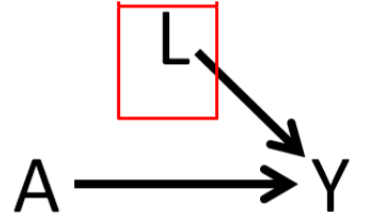
\includegraphics{images/RCT.png}

\hypertarget{parameters-of-interest}{%
\section{Parameters of interest}\label{parameters-of-interest}}

When assessing the effect of an exposure on an outcome, we are interested about the following estimands

\begin{itemize}
\tightlist
\item
  treatment effect for an individual (TE)
\item
  average treatment effect (ATE)
\item
  average treatment effect on the treated (ATT)
\end{itemize}

\hypertarget{te}{%
\subsection{TE}\label{te}}

\begin{itemize}
\tightlist
\item
  John takes Rosuvastatin \((A=1)\) and his total cholesterol level is = \(Y(A=1)\) = \(195\) mg/dL (milligrams per deciliter) after 3 months
\item
  John does not take Rosuvastatin \((A=0)\) and his total cholesterol level is = \(Y(A=0)\) = \(245\) mg/dL after 3 months
  Effect of Rosuvastatin on John is =
\end{itemize}

\(TE = Y(A=1) - Y(A=0) = 195 - 245 = - 50\)

\begin{tabular}{l>{}l}
\toprule
![](images/info.png) & \cellcolor[HTML]{3A3B3C}{\textcolor{white}{TE is not estimable as we generally can't observe outcomes under both treatment conditions.}}\\
\bottomrule
\end{tabular}

\hypertarget{ate}{%
\subsection{ATE}\label{ate}}

\begin{Shaded}
\begin{Highlighting}[]
\NormalTok{Person }\OtherTok{\textless{}{-}} \FunctionTok{c}\NormalTok{(}\StringTok{"John"}\NormalTok{,}\StringTok{"Jim"}\NormalTok{,}\StringTok{"Jake"}\NormalTok{,}\StringTok{"Cody"}\NormalTok{,}\StringTok{"Luke"}\NormalTok{)}
\NormalTok{Y1 }\OtherTok{\textless{}{-}} \FunctionTok{c}\NormalTok{( }\DecValTok{195}\NormalTok{, }\DecValTok{100}\NormalTok{, }\DecValTok{210}\NormalTok{, }\DecValTok{155}\NormalTok{, }\DecValTok{165}\NormalTok{)}
\NormalTok{Y0 }\OtherTok{\textless{}{-}} \FunctionTok{c}\NormalTok{(}\DecValTok{245}\NormalTok{, }\DecValTok{160}\NormalTok{, }\DecValTok{270}\NormalTok{, }\DecValTok{210}\NormalTok{, }\DecValTok{230}\NormalTok{)}
\NormalTok{PotentialOutcomes }\OtherTok{\textless{}{-}} \FunctionTok{data.frame}\NormalTok{(Person, Y1, Y0, }\AttributeTok{TE =}\NormalTok{ Y1}\SpecialCharTok{{-}}\NormalTok{Y0)}
\NormalTok{mean.values }\OtherTok{\textless{}{-}} \FunctionTok{c}\NormalTok{(}\ConstantTok{NA}\NormalTok{, }\FunctionTok{mean}\NormalTok{(PotentialOutcomes}\SpecialCharTok{$}\NormalTok{Y1),}
                 \FunctionTok{mean}\NormalTok{(PotentialOutcomes}\SpecialCharTok{$}\NormalTok{Y0),}
                 \FunctionTok{mean}\NormalTok{(PotentialOutcomes}\SpecialCharTok{$}\NormalTok{TE))}
\NormalTok{PotentialOutcomes }\OtherTok{\textless{}{-}} \FunctionTok{rbind}\NormalTok{(PotentialOutcomes, mean.values)}
\FunctionTok{kable}\NormalTok{(PotentialOutcomes, }\AttributeTok{booktabs =} \ConstantTok{TRUE}\NormalTok{, }
             \AttributeTok{col.names =} \FunctionTok{c}\NormalTok{(}\StringTok{"Person"}\NormalTok{, }\StringTok{"Y(1)"}\NormalTok{, }\StringTok{"Y(0)"}\NormalTok{, }\StringTok{"TE"}\NormalTok{)) }\SpecialCharTok{\%\textgreater{}\%}
  \FunctionTok{row\_spec}\NormalTok{(}\DecValTok{6}\NormalTok{, }\AttributeTok{bold =}\NormalTok{ T, }\AttributeTok{color =} \StringTok{"white"}\NormalTok{, }\AttributeTok{background =} \StringTok{"\#D7261E"}\NormalTok{)}
\end{Highlighting}
\end{Shaded}

\begin{tabular}{lrrr}
\toprule
Person & Y(1) & Y(0) & TE\\
\midrule
John & 195 & 245 & -50\\
Jim & 100 & 160 & -60\\
Jake & 210 & 270 & -60\\
Cody & 155 & 210 & -55\\
Luke & 165 & 230 & -65\\
\addlinespace
\cellcolor[HTML]{D7261E}{\textcolor{white}{\textbf{}}} & \cellcolor[HTML]{D7261E}{\textcolor{white}{\textbf{165}}} & \cellcolor[HTML]{D7261E}{\textcolor{white}{\textbf{223}}} & \cellcolor[HTML]{D7261E}{\textcolor{white}{\textbf{-58}}}\\
\bottomrule
\end{tabular}

\(ATE = E[Y(A=1)-Y(A=0)]\)

\begin{Shaded}
\begin{Highlighting}[]
\FunctionTok{mean}\NormalTok{(PotentialOutcomes}\SpecialCharTok{$}\NormalTok{Y1 }\SpecialCharTok{{-}}\NormalTok{ PotentialOutcomes}\SpecialCharTok{$}\NormalTok{Y0)}
\end{Highlighting}
\end{Shaded}

\begin{verbatim}
## [1] -58
\end{verbatim}

\hypertarget{interpretation-of-ate}{%
\subsection{Interpretation of ATE}\label{interpretation-of-ate}}

This is a treatment effect (on an average) of the following hypothetical situation

\begin{itemize}
\tightlist
\item
  having the entire population as treated, vs.
\item
  having the entire population as untreated.
\end{itemize}

Entire population is the reference goup here.

\hypertarget{identifiability-assumptions}{%
\subsection{Identifiability Assumptions}\label{identifiability-assumptions}}

If we can compute a causal quantity, such as \(ATE = E[Y(A=1)-Y(A=0)]\) using a statistical quantity, such as \texttt{mean(PotentialOutcomes\$Y1\ -\ PotentialOutcomes\$Y0)}, we say that the causal quantity is identifiable.

\begin{longtable}[]{@{}lll@{}}
\toprule
\endhead
\begin{minipage}[t]{(\columnwidth - 2\tabcolsep) * \real{0.33}}\raggedright
Exchangeability\strut
\end{minipage} & \begin{minipage}[t]{(\columnwidth - 2\tabcolsep) * \real{0.33}}\raggedright
\(Y(1), Y(0) \perp A\)\strut
\end{minipage} & \begin{minipage}[t]{(\columnwidth - 2\tabcolsep) * \real{0.33}}\raggedright
Treatment assignment is independent of the potential outcome\strut
\end{minipage}\tabularnewline
\begin{minipage}[t]{(\columnwidth - 2\tabcolsep) * \real{0.33}}\raggedright
Positivity\strut
\end{minipage} & \begin{minipage}[t]{(\columnwidth - 2\tabcolsep) * \real{0.33}}\raggedright
\(0 < P(A=1) < 1\)\strut
\end{minipage} & \begin{minipage}[t]{(\columnwidth - 2\tabcolsep) * \real{0.33}}\raggedright
Subjects are eligible to receive both treatment\strut
\end{minipage}\tabularnewline
\begin{minipage}[t]{(\columnwidth - 2\tabcolsep) * \real{0.33}}\raggedright
Consistency\strut
\end{minipage} & \begin{minipage}[t]{(\columnwidth - 2\tabcolsep) * \real{0.33}}\raggedright
\(Y = Y(a) \forall A=a\)\strut
\end{minipage} & \begin{minipage}[t]{(\columnwidth - 2\tabcolsep) * \real{0.33}}\raggedright
No multiple version of the treatment\strut
\end{minipage}\tabularnewline
\begin{minipage}[t]{(\columnwidth - 2\tabcolsep) * \real{0.33}}\raggedright
No interference\strut
\end{minipage} & \begin{minipage}[t]{(\columnwidth - 2\tabcolsep) * \real{0.33}}\raggedright
\strut
\end{minipage} & \begin{minipage}[t]{(\columnwidth - 2\tabcolsep) * \real{0.33}}\raggedright
Treated one patient will not impact outcome for others\strut
\end{minipage}\tabularnewline
\bottomrule
\end{longtable}

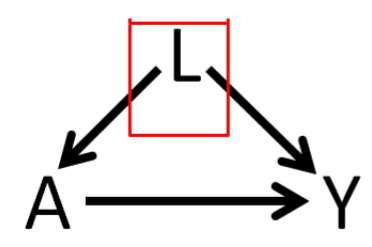
\includegraphics{images/condRCT.png}

Extending these assumptions when confounders exist:

\begin{longtable}[]{@{}lll@{}}
\toprule
\endhead
\begin{minipage}[t]{(\columnwidth - 2\tabcolsep) * \real{0.33}}\raggedright
Conditional Exchangeability\strut
\end{minipage} & \begin{minipage}[t]{(\columnwidth - 2\tabcolsep) * \real{0.33}}\raggedright
\(Y(1), Y(0) \perp A | L\)\strut
\end{minipage} & \begin{minipage}[t]{(\columnwidth - 2\tabcolsep) * \real{0.33}}\raggedright
Treatment assignment is independent of the potential outcome, given L\strut
\end{minipage}\tabularnewline
\begin{minipage}[t]{(\columnwidth - 2\tabcolsep) * \real{0.33}}\raggedright
Positivity\strut
\end{minipage} & \begin{minipage}[t]{(\columnwidth - 2\tabcolsep) * \real{0.33}}\raggedright
\(0 < P(A=1 | L) < 1\)\strut
\end{minipage} & \begin{minipage}[t]{(\columnwidth - 2\tabcolsep) * \real{0.33}}\raggedright
Subjects are eligible to receive both treatment, given L\strut
\end{minipage}\tabularnewline
\bottomrule
\end{longtable}

\hypertarget{att}{%
\subsection{ATT}\label{att}}

\begin{itemize}
\tightlist
\item
  Assume that the following are the confounders that impact the relationship between rosuvastatin and cholesterol levels

  \begin{itemize}
  \tightlist
  \item
    race
  \item
    sex
  \item
    age
  \end{itemize}
\item
  We have 5 Rosuvastatin-treated subjects who are all

  \begin{itemize}
  \tightlist
  \item
    white,
  \item
    male,
  \item
    50 years of age
  \end{itemize}
\item
  We recruited additional 5 subjects (same characteristics) to non-rosuvastatin group.
\end{itemize}

\textbf{Treated group}:

\begin{Shaded}
\begin{Highlighting}[]
\NormalTok{Person }\OtherTok{\textless{}{-}} \FunctionTok{c}\NormalTok{(}\StringTok{"John"}\NormalTok{,}\StringTok{"Jim"}\NormalTok{,}\StringTok{"Jake"}\NormalTok{,}\StringTok{"Cody"}\NormalTok{,}\StringTok{"Luke"}\NormalTok{)}
\NormalTok{Y1 }\OtherTok{\textless{}{-}} \FunctionTok{c}\NormalTok{( }\DecValTok{195}\NormalTok{, }\DecValTok{100}\NormalTok{, }\DecValTok{210}\NormalTok{, }\DecValTok{155}\NormalTok{, }\DecValTok{165}\NormalTok{)}
\NormalTok{Y0 }\OtherTok{\textless{}{-}} \FunctionTok{rep}\NormalTok{(}\ConstantTok{NA}\NormalTok{, }\FunctionTok{length}\NormalTok{(Y1))}
\NormalTok{Treated }\OtherTok{\textless{}{-}} \FunctionTok{data.frame}\NormalTok{(Person, Y1, Y0, }\AttributeTok{TE =}\NormalTok{ Y1}\SpecialCharTok{{-}}\NormalTok{Y0)}
\NormalTok{Treated[}\DecValTok{6}\NormalTok{,}\DecValTok{2}\NormalTok{] }\OtherTok{\textless{}{-}} \FunctionTok{mean}\NormalTok{(Treated}\SpecialCharTok{$}\NormalTok{Y1)}
\FunctionTok{kable}\NormalTok{(Treated, }\AttributeTok{booktabs =} \ConstantTok{TRUE}\NormalTok{, }
             \AttributeTok{col.names =} \FunctionTok{c}\NormalTok{(}\StringTok{"Person"}\NormalTok{, }\StringTok{"Y(1)"}\NormalTok{, }\StringTok{"Y(0)"}\NormalTok{, }\StringTok{"TE"}\NormalTok{))}\SpecialCharTok{\%\textgreater{}\%}
  \FunctionTok{row\_spec}\NormalTok{(}\DecValTok{6}\NormalTok{, }\AttributeTok{bold =}\NormalTok{ T, }\AttributeTok{color =} \StringTok{"white"}\NormalTok{, }\AttributeTok{background =} \StringTok{"\#D7261E"}\NormalTok{)}
\end{Highlighting}
\end{Shaded}

\begin{tabular}{lrlr}
\toprule
Person & Y(1) & Y(0) & TE\\
\midrule
John & 195 &  & \\
Jim & 100 &  & \\
Jake & 210 &  & \\
Cody & 155 &  & \\
Luke\cellcolor[HTML]{D7261E}{\textcolor{white}{\textbf{}}} & \cellcolor[HTML]{D7261E}{\textcolor{white}{\textbf{165}}} & \cellcolor[HTML]{D7261E}{\textcolor{white}{\textbf{}}} & \cellcolor[HTML]{D7261E}{\textcolor{white}{\textbf{}}}\\
\addlinespace
 & 165 &  & \\
\bottomrule
\end{tabular}

\textbf{Untreated group}: New folks with characteristics similar to the treated group.

\begin{Shaded}
\begin{Highlighting}[]
\NormalTok{Person }\OtherTok{\textless{}{-}} \FunctionTok{c}\NormalTok{( }\StringTok{"Jack"}\NormalTok{, }\StringTok{"Dustin"}\NormalTok{, }\StringTok{"Cole"}\NormalTok{, }\StringTok{"Lucas"}\NormalTok{, }\StringTok{"Dylan"}\NormalTok{)}
\NormalTok{Y0 }\OtherTok{\textless{}{-}} \FunctionTok{c}\NormalTok{( }\DecValTok{245}\NormalTok{, }\DecValTok{160}\NormalTok{, }\DecValTok{270}\NormalTok{, }\DecValTok{210}\NormalTok{, }\DecValTok{165}\NormalTok{)}
\NormalTok{Y1 }\OtherTok{\textless{}{-}} \FunctionTok{rep}\NormalTok{(}\ConstantTok{NA}\NormalTok{, }\FunctionTok{length}\NormalTok{(Y0))}
\NormalTok{Untreated }\OtherTok{\textless{}{-}} \FunctionTok{data.frame}\NormalTok{(Person, Y1, Y0, }\AttributeTok{TE =}\NormalTok{ Y1}\SpecialCharTok{{-}}\NormalTok{Y0)}
\NormalTok{Untreated[}\DecValTok{6}\NormalTok{,}\DecValTok{3}\NormalTok{] }\OtherTok{\textless{}{-}} \FunctionTok{mean}\NormalTok{(Untreated}\SpecialCharTok{$}\NormalTok{Y0)}
\FunctionTok{kable}\NormalTok{(Untreated, }\AttributeTok{booktabs =} \ConstantTok{TRUE}\NormalTok{, }
             \AttributeTok{col.names =} \FunctionTok{c}\NormalTok{(}\StringTok{"Person"}\NormalTok{, }\StringTok{"Y(1)"}\NormalTok{, }\StringTok{"Y(0)"}\NormalTok{, }\StringTok{"TE"}\NormalTok{))}\SpecialCharTok{\%\textgreater{}\%}
  \FunctionTok{row\_spec}\NormalTok{(}\DecValTok{6}\NormalTok{, }\AttributeTok{bold =}\NormalTok{ T, }\AttributeTok{color =} \StringTok{"white"}\NormalTok{, }\AttributeTok{background =} \StringTok{"\#D7261E"}\NormalTok{)}
\end{Highlighting}
\end{Shaded}

\begin{tabular}{llrr}
\toprule
Person & Y(1) & Y(0) & TE\\
\midrule
Jack &  & 245 & \\
Dustin &  & 160 & \\
Cole &  & 270 & \\
Lucas\cellcolor[HTML]{D7261E}{\textcolor{white}{\textbf{}}} & \cellcolor[HTML]{D7261E}{\textcolor{white}{\textbf{}}} & \cellcolor[HTML]{D7261E}{\textcolor{white}{\textbf{210}}} & \cellcolor[HTML]{D7261E}{\textcolor{white}{\textbf{}}}\\
Dylan &  & 165 & \\
\addlinespace
 &  & 210 & \\
\bottomrule
\end{tabular}

\(ATT = E[Y(A=1)-Y(A=0) | A = 1]\)

\begin{Shaded}
\begin{Highlighting}[]
\FunctionTok{mean}\NormalTok{(Treated}\SpecialCharTok{$}\NormalTok{Y1) }\SpecialCharTok{{-}} \FunctionTok{mean}\NormalTok{(Untreated}\SpecialCharTok{$}\NormalTok{Y0)}
\end{Highlighting}
\end{Shaded}

\begin{verbatim}
## [1] -45
\end{verbatim}

\hypertarget{interpretation-of-att}{%
\subsection{Interpretation of ATT}\label{interpretation-of-att}}

This is a treatment effect (on an average) of

\begin{itemize}
\tightlist
\item
  the treated population (reference group), vs.
\item
  untreated population, but have similar characteristics to the reference group/treated population.
\end{itemize}

It is also possible to change the reference population to untreated population. Then it is called Average Treatment Effect for the Untreated (ATU).

\hypertarget{att-vs.-ate}{%
\subsection{ATT vs.~ATE}\label{att-vs.-ate}}

\begin{tabular}{l>{}l}
\toprule
![](images/info.png) & \cellcolor[HTML]{3A3B3C}{\textcolor{white}{In a RCT (enough n), the ATT \& ATE are equivalent}}\\
![](images/info.png) & \cellcolor[HTML]{3A3B3C}{\textcolor{white}{In an observational study the ATT and ATE are not necessarily the same.}}\\
\bottomrule
\end{tabular}

\hypertarget{balance}{%
\section{Balance}\label{balance}}

\textbf{Balance in RCT}:

\begin{longtable}[]{@{}ll@{}}
\toprule
\endhead
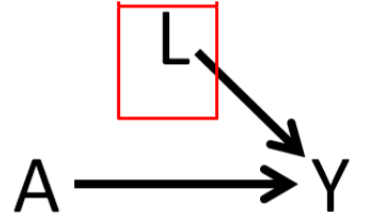
\includegraphics{images/RCT.png} & 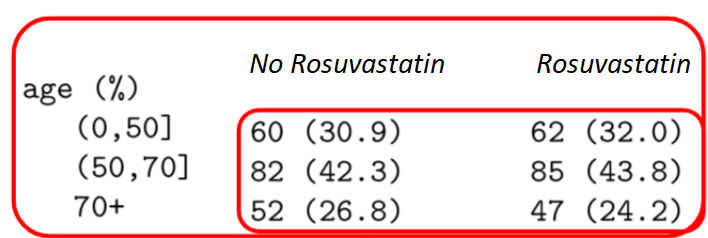
\includegraphics{images/balance.png}\tabularnewline
\bottomrule
\end{longtable}

\textbf{In absence of randomization}:

\begin{longtable}[]{@{}ll@{}}
\toprule
\endhead
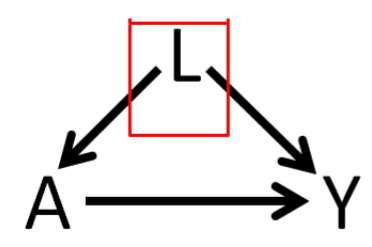
\includegraphics{images/condRCT.png} & 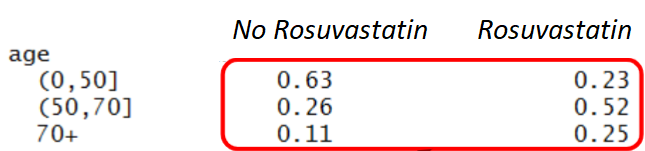
\includegraphics{images/imbalance.png}\tabularnewline
\bottomrule
\end{longtable}

\hypertarget{measures-of-balance}{%
\subsection{Measures of Balance}\label{measures-of-balance}}

\hypertarget{smd}{%
\subsubsection{SMD}\label{smd}}

\citet{austin2011introduction}

\begin{itemize}
\tightlist
\item
  For continuous confounders:

  \begin{itemize}
  \tightlist
  \item
    \(SDM_{continuous} = \frac{\bar{L}_{Rosuvastatin} - \bar{L}_{No Rosuvastatin}}{\sqrt{\frac{s^2_{Rosuvastatin} + s^2_{No Rosuvastatin}}{2}}}\)
  \end{itemize}
\item
  For binary confounders:

  \begin{itemize}
  \tightlist
  \item
    \(SDM_{binary} = \frac{\hat{p}_{Rosuvastatin} - \hat{p}_{No Rosuvastatin}}{\sqrt{\frac{ \hat{p}_{Rosuvastatin} \times (1 - \hat{p}_{Rosuvastatin}) + \hat{p}_{No Rosuvastatin} \times (1 - \hat{p}_{No Rosuvastatin}) }{2}}}\)
  \end{itemize}
\end{itemize}

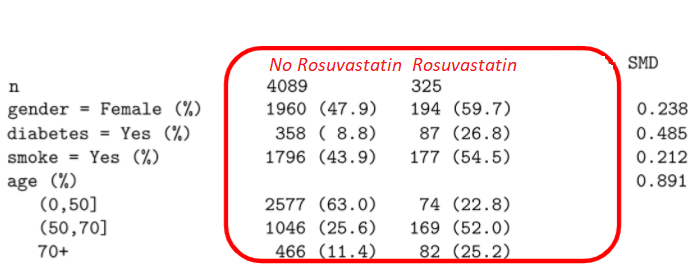
\includegraphics{images/SMD.png}

Generally, \(0.1\) is used as a cut-point. But some suggest more liberal cut-points. More on that later.

\textbf{COVID example} from \citet{gautret2020hydroxychloroquine}

p-value vs.~SMD

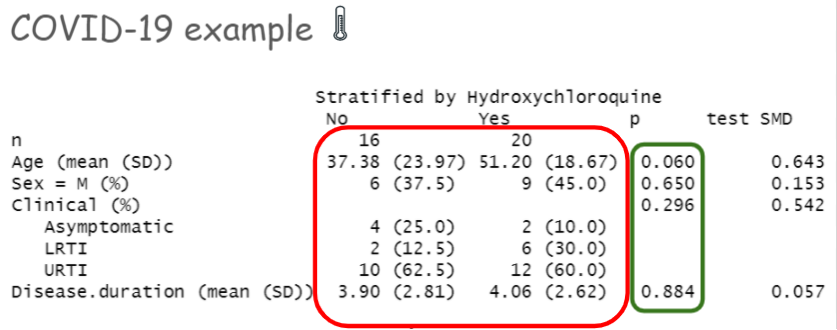
\includegraphics{images/hql.png}

\hypertarget{variance-ratio}{%
\subsubsection{Variance ratio}\label{variance-ratio}}

Variances of baseline characteristics between comparator groups under consideration. Suggested cut-point rages are (0.5 to 2). More liberal cutpoints are also used in the literature. More on this later.

\hypertarget{adjustment}{%
\section{Adjustment}\label{adjustment}}

\hypertarget{why-adjust}{%
\subsection{Why adjust?}\label{why-adjust}}

In absence of randomization, treatment effect estimate ATE = \(E[Y|A=1] - E[Y|A=0]\) includes

\begin{itemize}
\tightlist
\item
  Treatment effect
\item
  Systematic differences in 2 groups (`confounding')

  \begin{itemize}
  \tightlist
  \item
    Doctors may prescribe tx more to frail and older age patients.
  \item
    In here, \(L\) = age is a confounder.
  \end{itemize}
\end{itemize}

In absence of randomization, if age is a known confounder:

\begin{longtable}[]{@{}ll@{}}
\toprule
\endhead
\begin{minipage}[t]{(\columnwidth - 1\tabcolsep) * \real{0.50}}\raggedright
Causal effect for young (\(<50\))\strut
\end{minipage} & \begin{minipage}[t]{(\columnwidth - 1\tabcolsep) * \real{0.50}}\raggedright
\(E[Y|A=1, L =\) \texttt{younger\ age}\(]\) - \(E[Y|A=0, L =\) \texttt{younger\ age}\(]\)\strut
\end{minipage}\tabularnewline
\begin{minipage}[t]{(\columnwidth - 1\tabcolsep) * \real{0.50}}\raggedright
Causal effect for old (\(\ge 50\))\strut
\end{minipage} & \begin{minipage}[t]{(\columnwidth - 1\tabcolsep) * \real{0.50}}\raggedright
\(E[Y|A=1, L =\) \texttt{older\ age}\(]\) - \(E[Y|A=0, L =\) \texttt{older\ age}\(]\)\strut
\end{minipage}\tabularnewline
\bottomrule
\end{longtable}

Conditional exchangeability; only works if \(L\) is measured.

\hypertarget{adjustment-methods}{%
\subsection{Adjustment Methods}\label{adjustment-methods}}

Adjustment could mean

\begin{itemize}
\tightlist
\item
  exact matching
\item
  stratification
\end{itemize}

\begin{tabular}{l>{}l}
\toprule
![](images/info.png) & \cellcolor[HTML]{3A3B3C}{\textcolor{white}{When L includes a large number of covariates, matching method would result in a small sample size.}}\\
\bottomrule
\end{tabular}

Regression is also a popular adjustment method.

\hypertarget{overlap}{%
\section{Overlap}\label{overlap}}

\begin{itemize}
\tightlist
\item
  ``Lack of complete overlap'' happens if there is a baseline covariate space where there are exposed patients, but no control or vice versa.

  \begin{itemize}
  \tightlist
  \item
    Region of `no overlap' is an inherent limitation of the data.
  \end{itemize}
\end{itemize}

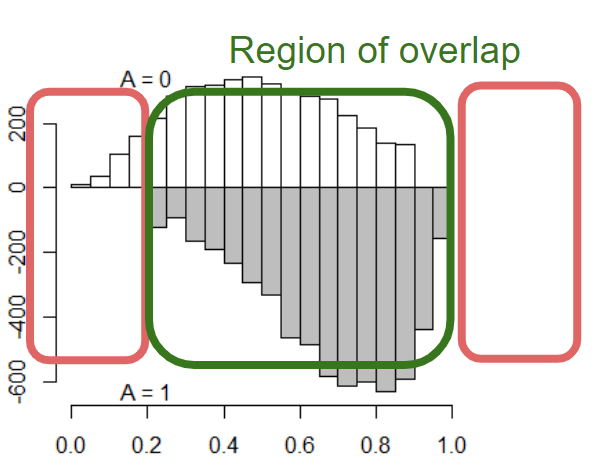
\includegraphics[width=8.47in]{images/overlap}

\begin{itemize}
\tightlist
\item
  \textbf{Regression adjustment} usually do not offer any solution to this.

  \begin{itemize}
  \tightlist
  \item
    Consequently, inference is not generalizable beyond the region of overlap.
  \end{itemize}
\end{itemize}

\hypertarget{ps}{%
\chapter{Propensity score}\label{ps}}

\hypertarget{motivating-problem}{%
\section{Motivating problem}\label{motivating-problem}}

\begin{longtable}[]{@{}ll@{}}
\toprule
\endhead
\(Y\) : Outcome & Cholesterol levels (high vs.~low)\tabularnewline
\(A\) : Exposure & Diabetes\tabularnewline
\(L\) : Known Confounders & gender, age, race, education, married, BMI\tabularnewline
\bottomrule
\end{longtable}

Search literature for the confounder variables, and look for those variables in the data source (\href{https://wwwn.cdc.gov/nchs/nhanes/continuousnhanes/default.aspx?BeginYear=2017}{NHANES 2017-2018}).

\begin{Shaded}
\begin{Highlighting}[]
\FunctionTok{load}\NormalTok{(}\AttributeTok{file=}\StringTok{"data/NHANES17.RData"}\NormalTok{) }
\FunctionTok{require}\NormalTok{(dplyr) }
\NormalTok{analytic }\OtherTok{\textless{}{-}}\NormalTok{ dplyr}\SpecialCharTok{::}\FunctionTok{select}\NormalTok{(analytic, }
\NormalTok{                  cholesterol, }\CommentTok{\# outcome}
\NormalTok{                  gender, age, race, education, }
\NormalTok{                  married, bmi, }\CommentTok{\# confounders}
\NormalTok{                  diabetes) }\CommentTok{\# exposure}
\NormalTok{analytic}\SpecialCharTok{$}\NormalTok{cholesterol }\OtherTok{\textless{}{-}} \FunctionTok{ifelse}\NormalTok{(analytic}\SpecialCharTok{$}\NormalTok{cholesterol }\SpecialCharTok{\textgreater{}} \DecValTok{240}\NormalTok{, }\DecValTok{1}\NormalTok{, }\DecValTok{0}\NormalTok{)}
\NormalTok{analytic}\SpecialCharTok{$}\NormalTok{diabetes }\OtherTok{\textless{}{-}} \FunctionTok{ifelse}\NormalTok{(analytic}\SpecialCharTok{$}\NormalTok{diabetes }\SpecialCharTok{==} \StringTok{"Yes"}\NormalTok{, }\DecValTok{1}\NormalTok{, }\DecValTok{0}\NormalTok{)}
\end{Highlighting}
\end{Shaded}

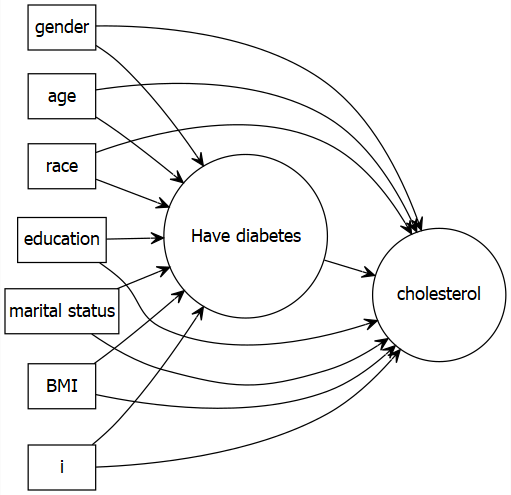
\includegraphics[width=0.65\linewidth]{images/overallnhanesplan}

\begin{Shaded}
\begin{Highlighting}[]
\FunctionTok{library}\NormalTok{(Hmisc)}
\end{Highlighting}
\end{Shaded}

\begin{verbatim}
## Loading required package: lattice
\end{verbatim}

\begin{verbatim}
## Loading required package: survival
\end{verbatim}

\begin{verbatim}
## Loading required package: Formula
\end{verbatim}

\begin{verbatim}
## Loading required package: ggplot2
\end{verbatim}

\begin{verbatim}
## 
## Attaching package: 'Hmisc'
\end{verbatim}

\begin{verbatim}
## The following object is masked from 'package:jtools':
## 
##     %nin%
\end{verbatim}

\begin{verbatim}
## The following objects are masked from 'package:dplyr':
## 
##     src, summarize
\end{verbatim}

\begin{verbatim}
## The following objects are masked from 'package:base':
## 
##     format.pval, units
\end{verbatim}

\begin{Shaded}
\begin{Highlighting}[]
\FunctionTok{describe}\NormalTok{(analytic)}
\end{Highlighting}
\end{Shaded}

\begin{verbatim}
## analytic 
## 
##  8  Variables      1562  Observations
## --------------------------------------------------------------------------------
## cholesterol 
##        n  missing distinct     Info      Sum     Mean      Gmd 
##     1562        0        2    0.292      171   0.1095   0.1951 
## 
## --------------------------------------------------------------------------------
## gender 
##        n  missing distinct 
##     1562        0        2 
##                         
## Value      Female   Male
## Frequency     603    959
## Proportion  0.386  0.614
## --------------------------------------------------------------------------------
## age : Age in years at screening 
##        n  missing distinct     Info     Mean      Gmd      .05      .10 
##     1562        0       61    0.999    53.18    19.78       25       29 
##      .25      .50      .75      .90      .95 
##       38       55       67       76       80 
## 
## lowest : 20 21 22 23 24, highest: 76 77 78 79 80
## --------------------------------------------------------------------------------
## race 
##        n  missing distinct 
##     1562        0        4 
##                                               
## Value         Black Hispanic    Other    White
## Frequency       324      284      228      726
## Proportion    0.207    0.182    0.146    0.465
## --------------------------------------------------------------------------------
## education 
##        n  missing distinct 
##     1562        0        3 
##                                               
## Value          College High.School      School
## Frequency          806         658          98
## Proportion       0.516       0.421       0.063
## --------------------------------------------------------------------------------
## married 
##        n  missing distinct 
##     1562        0        3 
##                                                                    
## Value                 Married      Never.married Previously.married
## Frequency                 921                228                413
## Proportion              0.590              0.146              0.264
## --------------------------------------------------------------------------------
## bmi : Body Mass Index (kg/m**2) 
##        n  missing distinct     Info     Mean      Gmd      .05      .10 
##     1562        0      314        1    29.96    7.972    20.00    21.71 
##      .25      .50      .75      .90      .95 
##    25.00    28.90    33.80    39.59    43.69 
## 
## lowest : 14.8 15.1 15.5 15.7 16.2, highest: 57.2 60.3 61.6 61.9 64.2
## --------------------------------------------------------------------------------
## diabetes 
##        n  missing distinct     Info      Sum     Mean      Gmd 
##     1562        0        2      0.5      330   0.2113   0.3335 
## 
## --------------------------------------------------------------------------------
\end{verbatim}

\hypertarget{defining-propensity-score}{%
\section{Defining Propensity score}\label{defining-propensity-score}}

\begin{itemize}
\tightlist
\item
  Conditional Probability of getting treatment, given the observed covariates
\end{itemize}

\begin{quote}
Prob(treatment: \(A = 1\) \textbar{} baseline or pre-treatment covariates: \(L\))
\end{quote}

\begin{quote}
Prob(\(A = 1\): Has diabetes \textbar{} \(L\): gender, age, race, education, married, bmi)
\end{quote}

\begin{itemize}
\tightlist
\item
  PS = \(Prob(A=1|L)\)
\end{itemize}

\hypertarget{theoretical-result}{%
\subsection{Theoretical result}\label{theoretical-result}}

\citet{rosenbaum1983central} showed:

\begin{itemize}
\tightlist
\item
  For potential outcomes \(Y(1), Y(0)\), if you have sufficient observed covariate list \(L\) to reduce confounding (`strong ignoribility'):

  \begin{itemize}
  \tightlist
  \item
    i.e., if \((Y(1), Y(0)) \perp A | L\)
  \item
    Note that is this NOT \(Y \perp A | L\)
  \end{itemize}
\item
  then

  \begin{itemize}
  \tightlist
  \item
    \((Y(1), Y(0)) \perp A | PS\) and
  \item
    \(A \perp L | PS\)
  \end{itemize}
\end{itemize}

\hypertarget{assumptions}{%
\subsection{Assumptions}\label{assumptions}}

\begin{longtable}[]{@{}lll@{}}
\toprule
\endhead
\begin{minipage}[t]{(\columnwidth - 2\tabcolsep) * \real{0.33}}\raggedright
Conditional Exchangeability\strut
\end{minipage} & \begin{minipage}[t]{(\columnwidth - 2\tabcolsep) * \real{0.33}}\raggedright
\(Y(1), Y(0) \perp A | L\)\strut
\end{minipage} & \begin{minipage}[t]{(\columnwidth - 2\tabcolsep) * \real{0.33}}\raggedright
Treatment assignment is independent of the potential outcome, given L\strut
\end{minipage}\tabularnewline
\begin{minipage}[t]{(\columnwidth - 2\tabcolsep) * \real{0.33}}\raggedright
Positivity\strut
\end{minipage} & \begin{minipage}[t]{(\columnwidth - 2\tabcolsep) * \real{0.33}}\raggedright
\(0 < P(A=1 | L) < 1\)\strut
\end{minipage} & \begin{minipage}[t]{(\columnwidth - 2\tabcolsep) * \real{0.33}}\raggedright
Subjects are eligible to receive both treatment, given L\strut
\end{minipage}\tabularnewline
\begin{minipage}[t]{(\columnwidth - 2\tabcolsep) * \real{0.33}}\raggedright
Consistency\strut
\end{minipage} & \begin{minipage}[t]{(\columnwidth - 2\tabcolsep) * \real{0.33}}\raggedright
\(Y = Y(a) \forall A=a\)\strut
\end{minipage} & \begin{minipage}[t]{(\columnwidth - 2\tabcolsep) * \real{0.33}}\raggedright
No multiple version of the treatment\strut
\end{minipage}\tabularnewline
\bottomrule
\end{longtable}

\hypertarget{ways-to-use-ps}{%
\subsection{Ways to use PS}\label{ways-to-use-ps}}

Many ways to use propensity scores (PS) in the analysis

\begin{itemize}
\tightlist
\item
  \textbf{PS matching} {[}our focus today: intuitive!{]}
\item
  PS weighting
\item
  PS stratification
\item
  PS used as a covariate
\end{itemize}

\hypertarget{ps-matching-steps}{%
\section{PS Matching Steps}\label{ps-matching-steps}}

Propensity score matching has 4 steps \citep{austin2011tutorial}

\begin{longtable}[]{@{}ll@{}}
\toprule
\endhead
Step 1 & exposure modelling: \(PS = Prob(A=1|L)\)\tabularnewline
Step 2 & Match by \(PS\)\tabularnewline
Step 3 & Assess balance and overlap (\(PS\) and \(L\))\tabularnewline
Step 4 & outcome modelling: \(Prob(Y=1|A=1)\)\tabularnewline
\bottomrule
\end{longtable}

\hypertarget{s1}{%
\chapter{Step 1: Exposure modelling}\label{s1}}

\hypertarget{model-specification}{%
\section{Model specification}\label{model-specification}}

Specify the propensity score model to estimate propensity scores, and fit the model:

\(A \sim L\)

\begin{Shaded}
\begin{Highlighting}[]
\NormalTok{baselinevars }\OtherTok{\textless{}{-}} \FunctionTok{c}\NormalTok{(}\StringTok{"gender"}\NormalTok{, }\StringTok{"age"}\NormalTok{, }\StringTok{"race"}\NormalTok{, }\StringTok{"education"}\NormalTok{, }\StringTok{"married"}\NormalTok{, }\StringTok{"bmi"}\NormalTok{)}
\NormalTok{ps.formula }\OtherTok{\textless{}{-}} \FunctionTok{as.formula}\NormalTok{(}\FunctionTok{paste}\NormalTok{(}\StringTok{"diabetes"}\NormalTok{, }\StringTok{"\textasciitilde{}"}\NormalTok{, }\FunctionTok{paste}\NormalTok{(baselinevars, }\AttributeTok{collapse =} \StringTok{"+"}\NormalTok{)))}
\NormalTok{ps.formula}
\end{Highlighting}
\end{Shaded}

\begin{verbatim}
## diabetes ~ gender + age + race + education + married + bmi
\end{verbatim}

\begin{Shaded}
\begin{Highlighting}[]
\CommentTok{\# fit logistic regression to estimate propensity scores}
\NormalTok{PS.fit }\OtherTok{\textless{}{-}} \FunctionTok{glm}\NormalTok{(ps.formula,}\AttributeTok{family=}\StringTok{"binomial"}\NormalTok{, }\AttributeTok{data=}\NormalTok{analytic)}
\FunctionTok{require}\NormalTok{(jtools)}
\FunctionTok{summ}\NormalTok{(PS.fit)}
\end{Highlighting}
\end{Shaded}

\begin{table}[!h]
\centering
\begin{tabular}{lr}
\toprule
\cellcolor{gray!6}{Observations} & \cellcolor{gray!6}{1562}\\
Dependent variable & diabetes\\
\cellcolor{gray!6}{Type} & \cellcolor{gray!6}{Generalized linear model}\\
Family & binomial\\
\cellcolor{gray!6}{Link} & \cellcolor{gray!6}{logit}\\
\bottomrule
\end{tabular}
\end{table} \begin{table}[!h]
\centering
\begin{tabular}{lr}
\toprule
\cellcolor{gray!6}{$\chi^2$(10)} & \cellcolor{gray!6}{282.89}\\
Pseudo-R² (Cragg-Uhler) & 0.26\\
\cellcolor{gray!6}{Pseudo-R² (McFadden)} & \cellcolor{gray!6}{0.18}\\
AIC & 1349.94\\
\cellcolor{gray!6}{BIC} & \cellcolor{gray!6}{1408.83}\\
\bottomrule
\end{tabular}
\end{table} \begin{table}[!h]
\centering
\begin{threeparttable}
\begin{tabular}{lrrrr}
\toprule
  & Est. & S.E. & z val. & p\\
\midrule
\cellcolor{gray!6}{(Intercept)} & \cellcolor{gray!6}{-8.38} & \cellcolor{gray!6}{0.58} & \cellcolor{gray!6}{-14.49} & \cellcolor{gray!6}{0.00}\\
genderMale & 0.34 & 0.15 & 2.26 & 0.02\\
\cellcolor{gray!6}{age} & \cellcolor{gray!6}{0.06} & \cellcolor{gray!6}{0.01} & \cellcolor{gray!6}{11.26} & \cellcolor{gray!6}{0.00}\\
raceHispanic & 0.15 & 0.23 & 0.64 & 0.52\\
\cellcolor{gray!6}{raceOther} & \cellcolor{gray!6}{0.76} & \cellcolor{gray!6}{0.23} & \cellcolor{gray!6}{3.25} & \cellcolor{gray!6}{0.00}\\
\addlinespace
raceWhite & -0.23 & 0.18 & -1.23 & 0.22\\
\cellcolor{gray!6}{educationHigh.School} & \cellcolor{gray!6}{0.14} & \cellcolor{gray!6}{0.15} & \cellcolor{gray!6}{0.95} & \cellcolor{gray!6}{0.34}\\
educationSchool & 0.52 & 0.27 & 1.92 & 0.05\\
\cellcolor{gray!6}{marriedNever.married} & \cellcolor{gray!6}{-0.04} & \cellcolor{gray!6}{0.25} & \cellcolor{gray!6}{-0.16} & \cellcolor{gray!6}{0.88}\\
marriedPreviously.married & -0.02 & 0.16 & -0.15 & 0.88\\
\addlinespace
\cellcolor{gray!6}{bmi} & \cellcolor{gray!6}{0.10} & \cellcolor{gray!6}{0.01} & \cellcolor{gray!6}{10.14} & \cellcolor{gray!6}{0.00}\\
\bottomrule
\end{tabular}
\begin{tablenotes}
\item Standard errors: MLE
\end{tablenotes}
\end{threeparttable}
\end{table}

\begin{itemize}
\tightlist
\item
  Coef of PS model fit is not of concern
\item
  Model can be rich: to the extent that prediction is better
\item
  But look for multi-collinearity issues

  \begin{itemize}
  \tightlist
  \item
    SE too high?
  \end{itemize}
\end{itemize}

\hypertarget{variables-to-adjust}{%
\section{Variables to adjust}\label{variables-to-adjust}}

\citet{brookhart2006variable}

\begin{itemize}
\tightlist
\item
  Observed covariates are used to fix design
\item
  Which covariates should be selected:

  \begin{itemize}
  \tightlist
  \item
    known to be a confounder (causes of \(Y\) and \(A\))
  \item
    known to be a cause of the outcome (risk factors of \(Y\))
  \item
    avoid known instruments or noise variables: \textbf{SE suffers}
  \item
    mediating factors should be avoided (total effect = goal)
  \end{itemize}
\item
  Try drawing \href{http://www.dagitty.net/}{causal diagram} to determine which variables to include
\end{itemize}

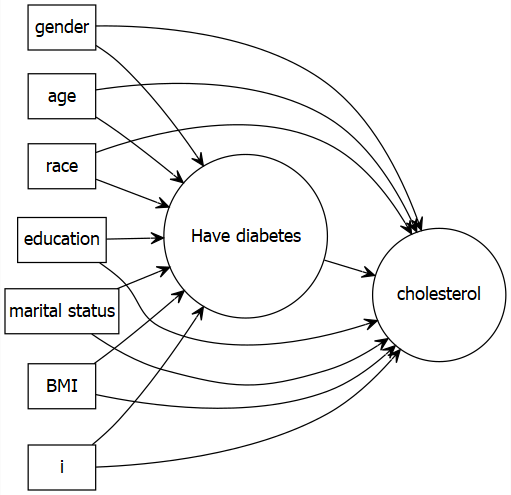
\includegraphics[width=0.65\linewidth]{images/overallnhanesplan}

\hypertarget{model-selection}{%
\section{Model selection}\label{model-selection}}

Usually done for the variables that are \emph{not known as a confounder} in the literature, or based on subject area knowledge.

\begin{itemize}
\tightlist
\item
  Stepwise (p-value or criterion based) not recommended

  \begin{itemize}
  \tightlist
  \item
    depending on sample size, different values can get selected
  \item
    may select variables highly associated with \(A\)
  \end{itemize}
\item
  Don't look at the outcome (\(Y\)) in your data to select covariates

  \begin{itemize}
  \tightlist
  \item
    There are debate about this (ideal vs.~pragmatism)
  \item
    see \citet{karim2018can} for an example.
  \end{itemize}
\end{itemize}

\hypertarget{alternative-modelling-strategies}{%
\section{Alternative modelling strategies}\label{alternative-modelling-strategies}}

\begin{itemize}
\tightlist
\item
  Other machine learning alternatives are possible to use instead of logistic regression.

  \begin{itemize}
  \tightlist
  \item
    tree based methods have better ability to detect non-linearity / non-additivity (\textbf{model-specification} aspect)
  \item
    shrinkage methods - lasso / elastic net may better deal with multi-collinearity
  \item
    ensemble learners / super learners were successfully used
  \item
    shallow/deep learning!
  \end{itemize}
\end{itemize}

\hypertarget{ps-estimation}{%
\section{PS estimation}\label{ps-estimation}}

PS is unknown, and needs to be estimated from the fitted exposure model:

\begin{Shaded}
\begin{Highlighting}[]
\CommentTok{\# extract estimated propensity scores from the fit}
\NormalTok{analytic}\SpecialCharTok{$}\NormalTok{PS }\OtherTok{\textless{}{-}} \FunctionTok{predict}\NormalTok{(PS.fit, }\AttributeTok{newdata =}\NormalTok{ analytic, }\AttributeTok{type=}\StringTok{"response"}\NormalTok{)}
\end{Highlighting}
\end{Shaded}

\begin{Shaded}
\begin{Highlighting}[]
\FunctionTok{require}\NormalTok{(cobalt)}
\FunctionTok{bal.plot}\NormalTok{(analytic, }\AttributeTok{var.name =} \StringTok{"PS"}\NormalTok{, }
         \AttributeTok{treat =} \StringTok{"diabetes"}\NormalTok{, }
         \AttributeTok{which =} \StringTok{"both"}\NormalTok{, }
         \AttributeTok{data =}\NormalTok{ analytic)}
\end{Highlighting}
\end{Shaded}

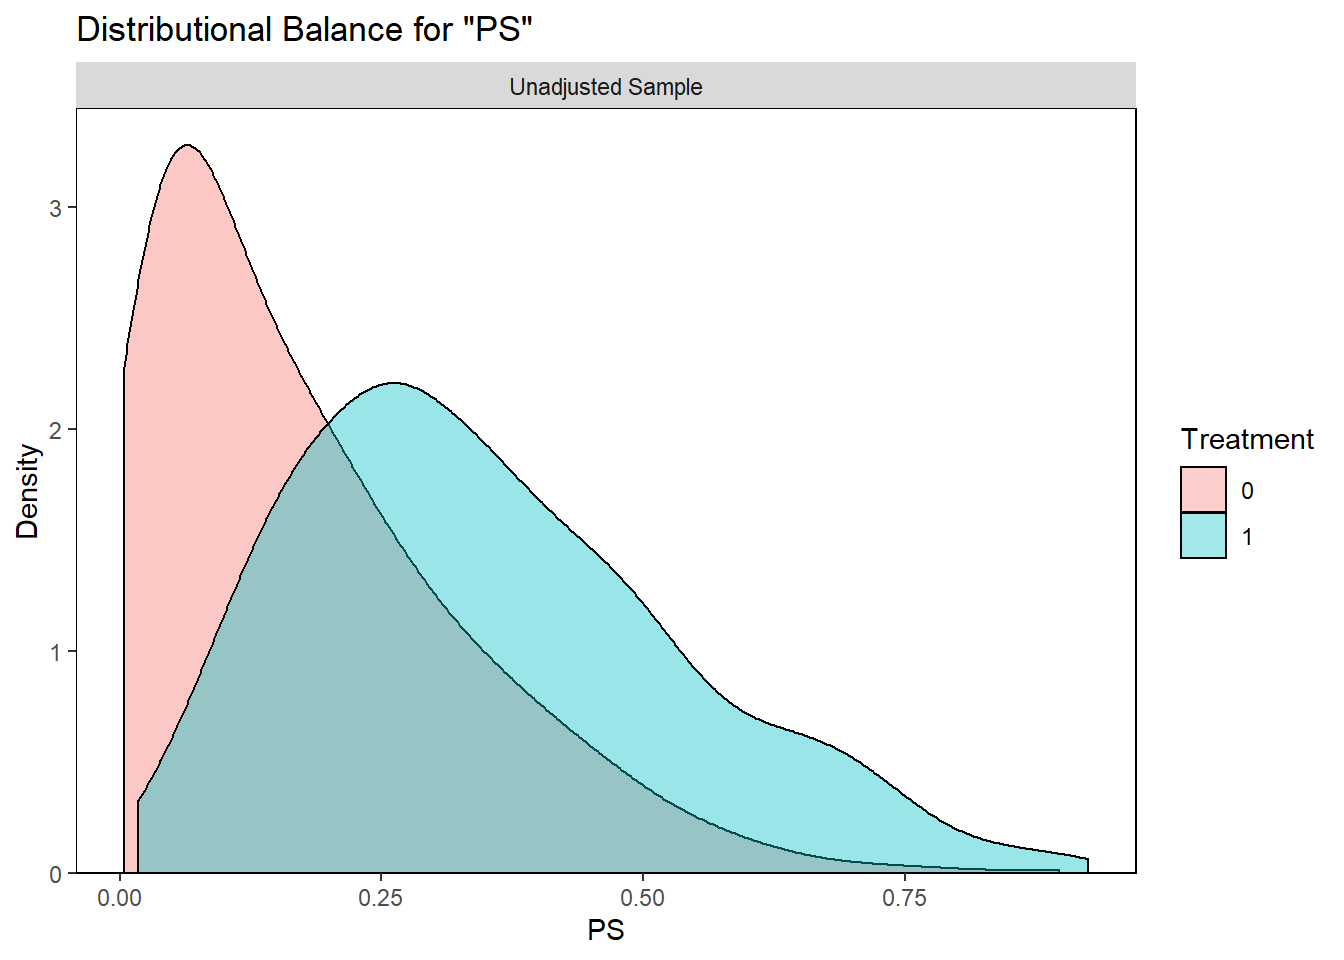
\includegraphics{UnderstandingPropensityScore_files/figure-latex/ps2cc-1.pdf}

\begin{tabular}{l>{}l}
\toprule
![](images/info.png) & \cellcolor[HTML]{3A3B3C}{\textcolor{white}{Don't loose sight that better **balance** is the ultimate goal for propensity score}}\\
![](images/info.png) & \cellcolor[HTML]{3A3B3C}{\textcolor{white}{Prediction of \$A\$ is just a means to that end (as true PS is unknown)}}\\
![](images/info.png) & \cellcolor[HTML]{3A3B3C}{\textcolor{white}{May attract variables highly associated with \$A\$}}\\
\bottomrule
\end{tabular}

\hypertarget{s2}{%
\chapter{Step 2: Propensity score Matching}\label{s2}}

\hypertarget{matching-method-nn}{%
\section{Matching method NN}\label{matching-method-nn}}

Match using estimates propensity scores

\begin{itemize}
\tightlist
\item
  nearest-neighbor (NN) matching
\item
  without replacement
\item
  with caliper = .2*SD of logit of propensity score
\item
  with 1:1 ratio (pair-matching)
\end{itemize}

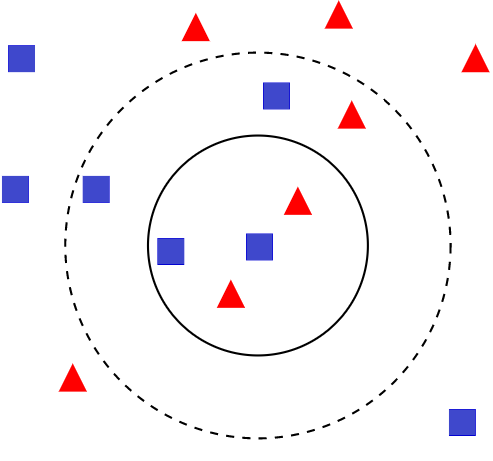
\includegraphics[width=0.5\linewidth]{images/nn}

\hypertarget{initial-fit}{%
\section{Initial fit}\label{initial-fit}}

1:1 NN Match using estimates propensity scores

\begin{Shaded}
\begin{Highlighting}[]
\FunctionTok{set.seed}\NormalTok{(}\DecValTok{123}\NormalTok{)}
\FunctionTok{require}\NormalTok{(MatchIt)}
\NormalTok{match.obj }\OtherTok{\textless{}{-}} \FunctionTok{matchit}\NormalTok{(ps.formula, }\AttributeTok{data =}\NormalTok{ analytic,}
                     \AttributeTok{distance =} \StringTok{\textquotesingle{}logit\textquotesingle{}}\NormalTok{, }
                     \AttributeTok{method =} \StringTok{"nearest"}\NormalTok{, }
                     \AttributeTok{replace=}\ConstantTok{FALSE}\NormalTok{,}
                     \AttributeTok{ratio =} \DecValTok{1}\NormalTok{)}
\NormalTok{analytic}\SpecialCharTok{$}\NormalTok{PS }\OtherTok{\textless{}{-}}\NormalTok{ match.obj}\SpecialCharTok{$}\NormalTok{distance}
\FunctionTok{summary}\NormalTok{(match.obj}\SpecialCharTok{$}\NormalTok{distance)}
\end{Highlighting}
\end{Shaded}

\begin{verbatim}
##     Min.  1st Qu.   Median     Mean  3rd Qu.     Max. 
## 0.003916 0.068128 0.169946 0.211268 0.312987 0.925132
\end{verbatim}

\begin{Shaded}
\begin{Highlighting}[]
\NormalTok{match.obj}
\end{Highlighting}
\end{Shaded}

\begin{verbatim}
## A matchit object
##  - method: 1:1 nearest neighbor matching without replacement
##  - distance: Propensity score
##              - estimated with logistic regression
##  - number of obs.: 1562 (original), 660 (matched)
##  - target estimand: ATT
##  - covariates: gender, age, race, education, married, bmi
\end{verbatim}

\hypertarget{fine-tuning-add-caliper}{%
\section{Fine tuning: add caliper}\label{fine-tuning-add-caliper}}

2 SD of logit of the propensity score is suggested as a caliper.

\begin{Shaded}
\begin{Highlighting}[]
\NormalTok{logitPS }\OtherTok{\textless{}{-}}  \SpecialCharTok{{-}}\FunctionTok{log}\NormalTok{(}\DecValTok{1}\SpecialCharTok{/}\NormalTok{analytic}\SpecialCharTok{$}\NormalTok{PS }\SpecialCharTok{{-}} \DecValTok{1}\NormalTok{) }
\CommentTok{\# logit of the propensity score}
\NormalTok{.}\DecValTok{2}\SpecialCharTok{*}\FunctionTok{sd}\NormalTok{(logitPS) }\CommentTok{\# suggested in the literature}
\end{Highlighting}
\end{Shaded}

\begin{verbatim}
## [1] 0.2606266
\end{verbatim}

\begin{Shaded}
\begin{Highlighting}[]
\CommentTok{\# choosing too strict PS has unintended consequences }
\end{Highlighting}
\end{Shaded}

\begin{Shaded}
\begin{Highlighting}[]
\FunctionTok{set.seed}\NormalTok{(}\DecValTok{123}\NormalTok{)}
\FunctionTok{require}\NormalTok{(MatchIt)}
\NormalTok{match.obj }\OtherTok{\textless{}{-}} \FunctionTok{matchit}\NormalTok{(ps.formula, }\AttributeTok{data =}\NormalTok{ analytic,}
                     \AttributeTok{distance =} \StringTok{\textquotesingle{}logit\textquotesingle{}}\NormalTok{, }
                     \AttributeTok{method =} \StringTok{"nearest"}\NormalTok{, }
                     \AttributeTok{replace=}\ConstantTok{FALSE}\NormalTok{,}
                     \AttributeTok{caliper =}\NormalTok{ .}\DecValTok{2}\SpecialCharTok{*}\FunctionTok{sd}\NormalTok{(logitPS), }
                     \AttributeTok{ratio =} \DecValTok{1}\NormalTok{)}
\NormalTok{analytic}\SpecialCharTok{$}\NormalTok{PS }\OtherTok{\textless{}{-}}\NormalTok{ match.obj}\SpecialCharTok{$}\NormalTok{distance}
\FunctionTok{summary}\NormalTok{(match.obj}\SpecialCharTok{$}\NormalTok{distance)}
\end{Highlighting}
\end{Shaded}

\begin{verbatim}
##     Min.  1st Qu.   Median     Mean  3rd Qu.     Max. 
## 0.003916 0.068128 0.169946 0.211268 0.312987 0.925132
\end{verbatim}

\begin{Shaded}
\begin{Highlighting}[]
\NormalTok{match.obj}
\end{Highlighting}
\end{Shaded}

\begin{verbatim}
## A matchit object
##  - method: 1:1 nearest neighbor matching without replacement
##  - distance: Propensity score [caliper]
##              - estimated with logistic regression
##  - caliper: <distance> (0.045)
##  - number of obs.: 1562 (original), 632 (matched)
##  - target estimand: ATT
##  - covariates: gender, age, race, education, married, bmi
\end{verbatim}

\hypertarget{matches}{%
\section{Matches}\label{matches}}

Taking a closer look at the matches

\begin{Shaded}
\begin{Highlighting}[]
\CommentTok{\# Ref: https://lists.gking.harvard.edu/pipermail/matchit/2013{-}October/000559.html}
\NormalTok{matches }\OtherTok{\textless{}{-}} \FunctionTok{as.data.frame}\NormalTok{(match.obj}\SpecialCharTok{$}\NormalTok{match.matrix)}
\FunctionTok{colnames}\NormalTok{(matches)}\OtherTok{\textless{}{-}}\FunctionTok{c}\NormalTok{(}\StringTok{"matched\_unit"}\NormalTok{)}
\NormalTok{matches}\SpecialCharTok{$}\NormalTok{matched\_unit}\OtherTok{\textless{}{-}}\FunctionTok{as.numeric}\NormalTok{(}
  \FunctionTok{as.character}\NormalTok{(matches}\SpecialCharTok{$}\NormalTok{matched\_unit))}
\NormalTok{matches}\SpecialCharTok{$}\NormalTok{treated\_unit}\OtherTok{\textless{}{-}}\FunctionTok{as.numeric}\NormalTok{(}\FunctionTok{rownames}\NormalTok{(matches))}
\NormalTok{matches.only}\OtherTok{\textless{}{-}}\NormalTok{matches[}\SpecialCharTok{!}\FunctionTok{is.na}\NormalTok{(matches}\SpecialCharTok{$}\NormalTok{matched\_unit),]}
\FunctionTok{head}\NormalTok{(matches.only)}
\end{Highlighting}
\end{Shaded}

\begin{verbatim}
##     matched_unit treated_unit
## 40          8496           40
## 56          3139           56
## 65          4192           65
## 66            94           66
## 86          2212           86
## 110         7154          110
\end{verbatim}

\hypertarget{other-matching-algorithms}{%
\section{Other matching algorithms}\label{other-matching-algorithms}}

More NN ratio is usually better. But creates issue when calculating variances (but can be easily handled).

Other possibilities

\begin{itemize}
\tightlist
\item
  Optimal
\item
  genetic matching
\item
  CEM
\item
  variable ratio NN
\end{itemize}

\hypertarget{s3}{%
\chapter{Step 3: Balance and overlap}\label{s3}}

\textbf{Balance is more important than prediction}!

\begin{itemize}
\tightlist
\item
  Criteria to assess success of step 2: PS estimation

  \begin{itemize}
  \tightlist
  \item
    better balance
  \item
    better overlap {[}no extrapolation!{]}
  \item
    PS = 0 or PS = 1 needs close inspection
  \end{itemize}
\end{itemize}

\hypertarget{assessment-of-balance-by-smd}{%
\section{Assessment of Balance by SMD}\label{assessment-of-balance-by-smd}}

\begin{itemize}
\tightlist
\item
  balance = similarity of the covariate distributions
\item
  \(d\) or \(SMD > 0.1\) can be considered as imbalance \citep{austin2011introduction}
\end{itemize}

\begin{Shaded}
\begin{Highlighting}[]
\NormalTok{tab1e }\OtherTok{\textless{}{-}} \FunctionTok{CreateTableOne}\NormalTok{(}\AttributeTok{vars =}\NormalTok{ baselinevars,}
                        \AttributeTok{data =}\NormalTok{ analytic, }
                        \AttributeTok{strata =} \StringTok{"diabetes"}\NormalTok{,}
                        \AttributeTok{includeNA =} \ConstantTok{TRUE}\NormalTok{,}
                        \AttributeTok{test =} \ConstantTok{TRUE}\NormalTok{, }\AttributeTok{smd =} \ConstantTok{TRUE}\NormalTok{)}
\FunctionTok{print}\NormalTok{(tab1e, }\AttributeTok{showAllLevels =} \ConstantTok{FALSE}\NormalTok{, }\AttributeTok{smd =} \ConstantTok{TRUE}\NormalTok{, }\AttributeTok{test =} \ConstantTok{TRUE}\NormalTok{)}
\end{Highlighting}
\end{Shaded}

\begin{verbatim}
##                        Stratified by diabetes
##                         0             1             p      test SMD   
##   n                      1232           330                           
##   gender = Male (%)       738 (59.9)    221 (67.0)   0.023       0.147
##   age (mean (SD))       50.54 (17.23) 63.04 (12.87) <0.001       0.822
##   race (%)                                           0.110       0.151
##      Black                253 (20.5)     71 (21.5)                    
##      Hispanic             220 (17.9)     64 (19.4)                    
##      Other                169 (13.7)     59 (17.9)                    
##      White                590 (47.9)    136 (41.2)                    
##   education (%)                                      0.005       0.186
##      College              649 (52.7)    157 (47.6)                    
##      High.School          518 (42.0)    140 (42.4)                    
##      School                65 ( 5.3)     33 (10.0)                    
##   married (%)                                       <0.001       0.282
##      Married              727 (59.0)    194 (58.8)                    
##      Never.married        201 (16.3)     27 ( 8.2)                    
##      Previously.married   304 (24.7)    109 (33.0)                    
##   bmi (mean (SD))       29.14 (7.03)  33.01 (7.65)  <0.001       0.526
\end{verbatim}

\hypertarget{vizualization-for-overlap}{%
\section{Vizualization for Overlap}\label{vizualization-for-overlap}}

\begin{Shaded}
\begin{Highlighting}[]
\FunctionTok{boxplot}\NormalTok{(PS }\SpecialCharTok{\textasciitilde{}}\NormalTok{ diabetes, }\AttributeTok{data =}\NormalTok{ analytic, }
        \AttributeTok{lwd =} \DecValTok{2}\NormalTok{, }\AttributeTok{ylab =} \StringTok{\textquotesingle{}PS\textquotesingle{}}\NormalTok{)}
\FunctionTok{stripchart}\NormalTok{(PS }\SpecialCharTok{\textasciitilde{}}\NormalTok{ diabetes, }\AttributeTok{vertical =} \ConstantTok{TRUE}\NormalTok{, }
           \AttributeTok{data =}\NormalTok{ analytic, }\AttributeTok{method =} \StringTok{"jitter"}\NormalTok{, }
           \AttributeTok{add =} \ConstantTok{TRUE}\NormalTok{, }\AttributeTok{pch =} \DecValTok{20}\NormalTok{, }\AttributeTok{col =} \StringTok{\textquotesingle{}blue\textquotesingle{}}\NormalTok{)}
\end{Highlighting}
\end{Shaded}

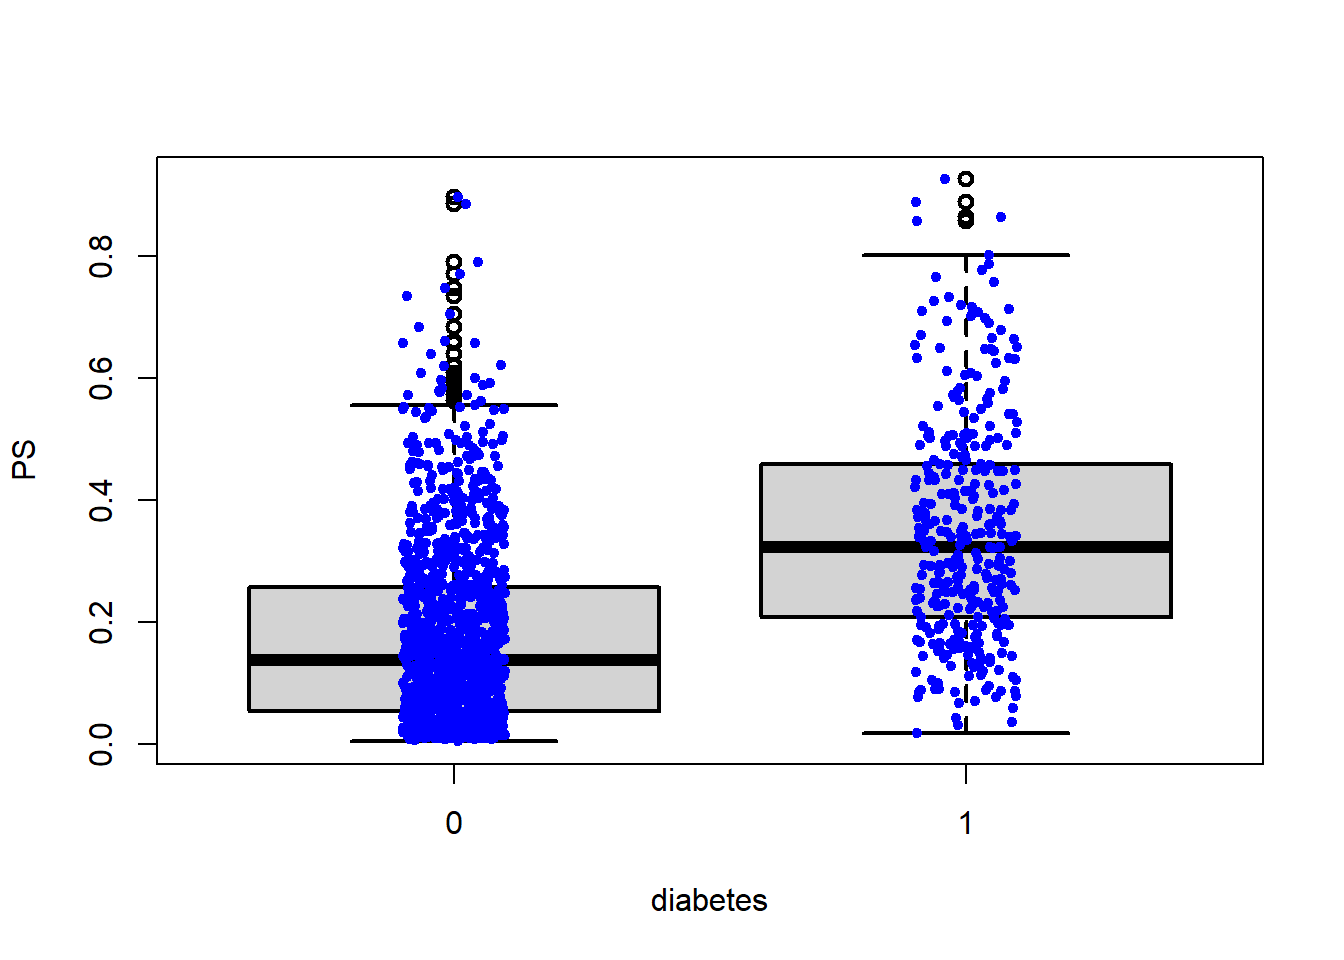
\includegraphics[width=0.3\linewidth]{UnderstandingPropensityScore_files/figure-latex/ps3vv-1}

\begin{Shaded}
\begin{Highlighting}[]
\FunctionTok{plot}\NormalTok{(match.obj, }\AttributeTok{type =} \StringTok{"jitter"}\NormalTok{)}
\end{Highlighting}
\end{Shaded}

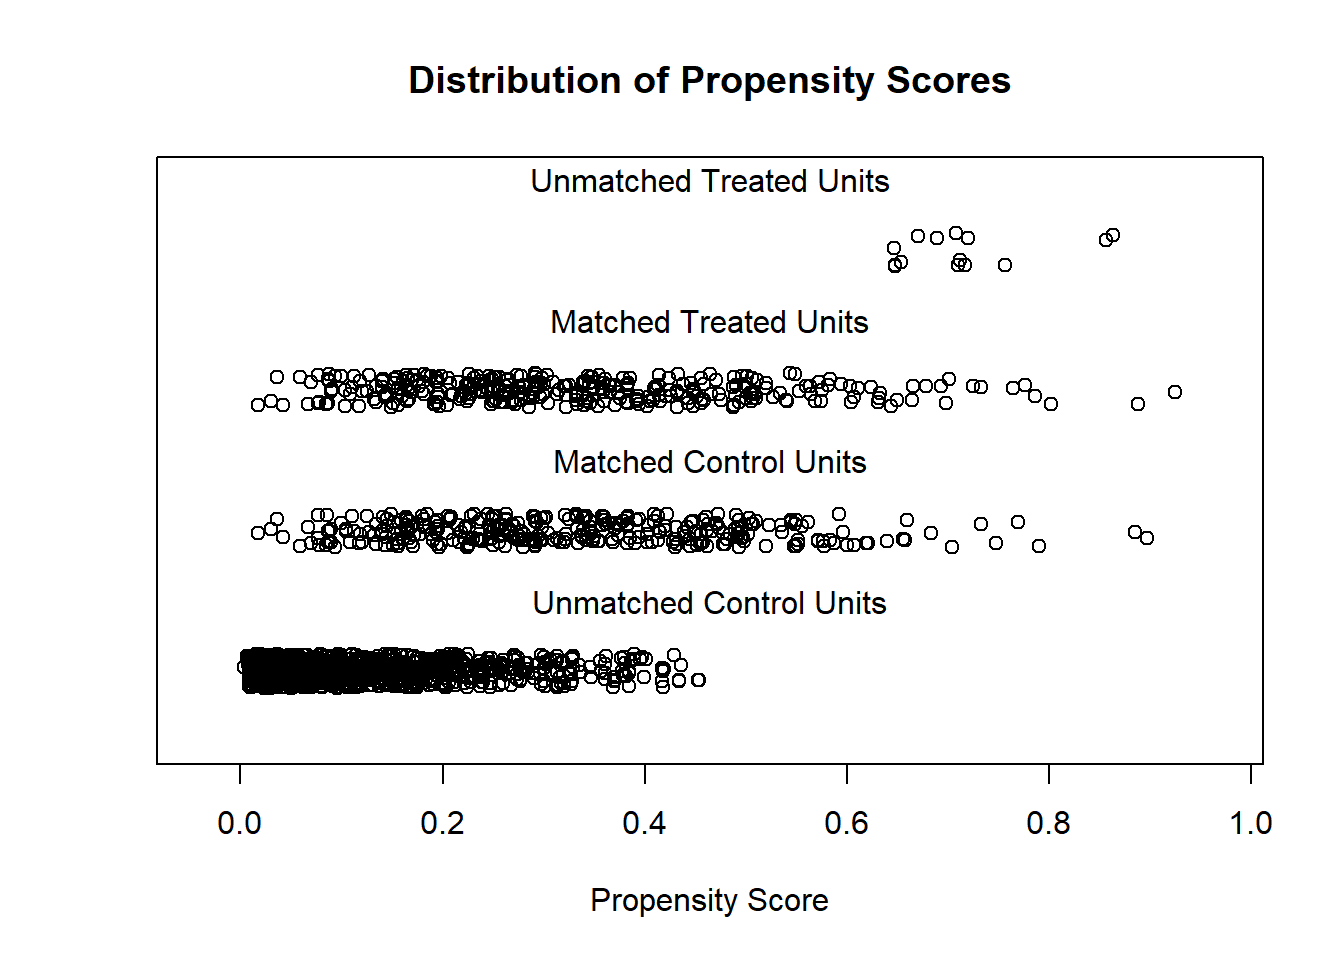
\includegraphics[width=0.5\linewidth]{UnderstandingPropensityScore_files/figure-latex/ps8vv-1}

\begin{verbatim}
## [1] "To identify the units, use first mouse button; to stop, use second."
\end{verbatim}

\begin{verbatim}
## integer(0)
\end{verbatim}

Vizualization for assessing overlap issues

\begin{Shaded}
\begin{Highlighting}[]
\FunctionTok{plot}\NormalTok{(match.obj, }\AttributeTok{type =} \StringTok{"hist"}\NormalTok{)}
\end{Highlighting}
\end{Shaded}

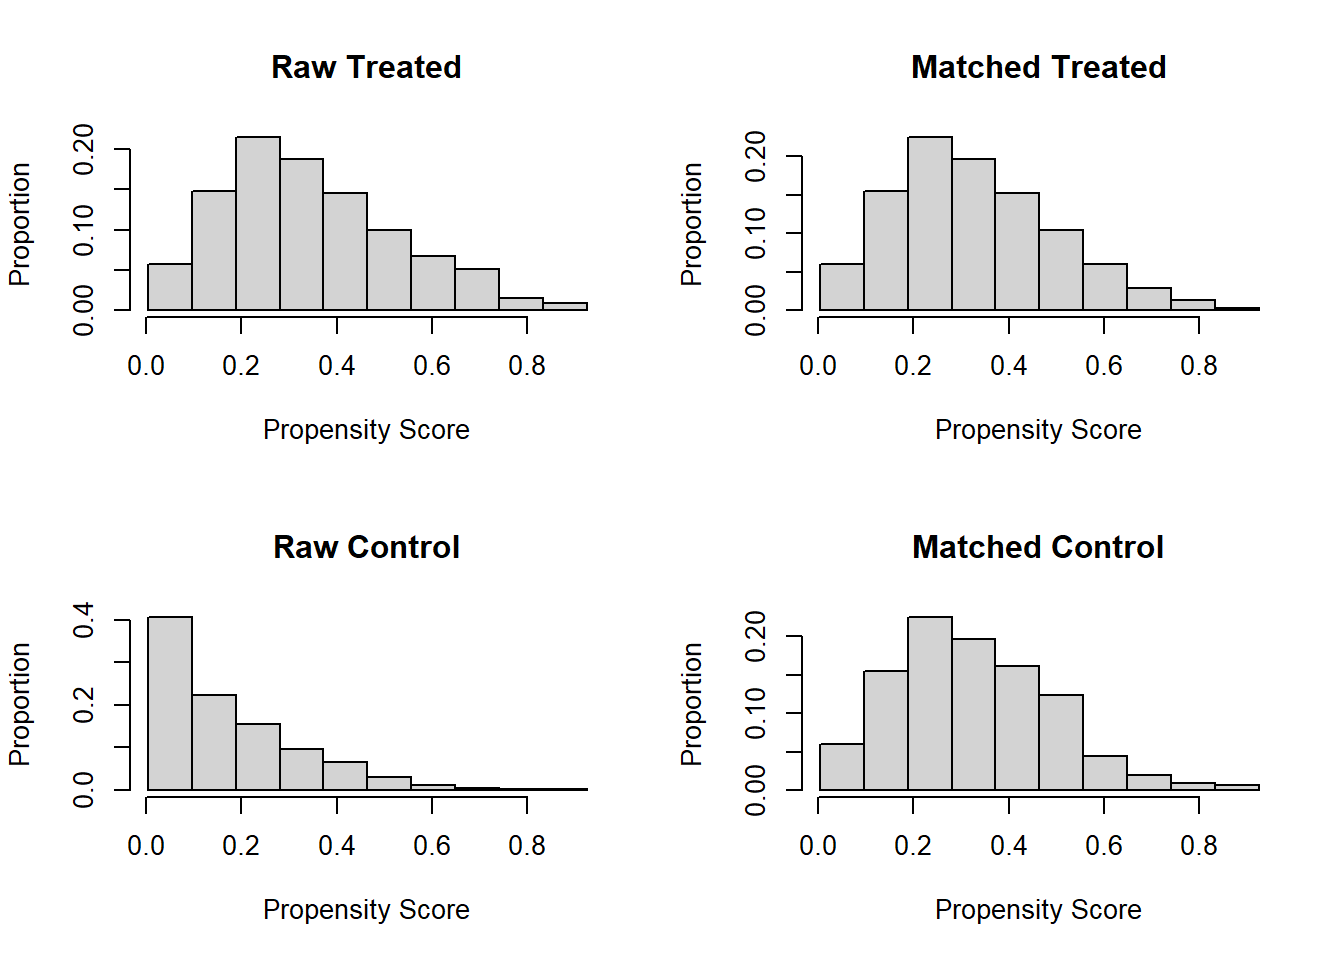
\includegraphics[width=0.5\linewidth]{UnderstandingPropensityScore_files/figure-latex/ps9vv-1}

Assessment of Balance: Better than regression diagnostics!

\begin{Shaded}
\begin{Highlighting}[]
\NormalTok{matched.data }\OtherTok{\textless{}{-}} \FunctionTok{match.data}\NormalTok{(match.obj)}
\NormalTok{tab1m }\OtherTok{\textless{}{-}} \FunctionTok{CreateTableOne}\NormalTok{(}\AttributeTok{vars =}\NormalTok{ baselinevars, }
                        \AttributeTok{strata =} \StringTok{"diabetes"}\NormalTok{, }
                        \AttributeTok{data =}\NormalTok{ matched.data, }
                        \AttributeTok{includeNA =} \ConstantTok{TRUE}\NormalTok{, }
                        \AttributeTok{test =} \ConstantTok{TRUE}\NormalTok{, }\AttributeTok{smd =} \ConstantTok{TRUE}\NormalTok{)}
\end{Highlighting}
\end{Shaded}

Compare the similarity of baseline characteristics between treated and untreated subjects in a the propensity score-matched sample.

\begin{itemize}
\tightlist
\item
  In this case, we will compare SMD \textless{} 0.1 or not.
\item
  In some literature, other generous values (0.25) are proposed. \citep{austin2011introduction}
\end{itemize}

\begin{Shaded}
\begin{Highlighting}[]
\FunctionTok{print}\NormalTok{(tab1m, }\AttributeTok{showAllLevels =} \ConstantTok{FALSE}\NormalTok{, }\AttributeTok{smd =} \ConstantTok{TRUE}\NormalTok{, }\AttributeTok{test =} \ConstantTok{FALSE}\NormalTok{) }
\end{Highlighting}
\end{Shaded}

\begin{verbatim}
##                        Stratified by diabetes
##                         0             1             SMD   
##   n                       316           316               
##   gender = Male (%)       218 (69.0)    212 (67.1)   0.041
##   age (mean (SD))       63.03 (13.48) 62.67 (12.87)  0.027
##   race (%)                                           0.105
##      Black                 79 (25.0)     68 (21.5)        
##      Hispanic              58 (18.4)     61 (19.3)        
##      Other                 44 (13.9)     53 (16.8)        
##      White                135 (42.7)    134 (42.4)        
##   education (%)                                      0.007
##      College              153 (48.4)    152 (48.1)        
##      High.School          133 (42.1)    134 (42.4)        
##      School                30 ( 9.5)     30 ( 9.5)        
##   married (%)                                        0.099
##      Married              183 (57.9)    186 (58.9)        
##      Never.married         20 ( 6.3)     27 ( 8.5)        
##      Previously.married   113 (35.8)    103 (32.6)        
##   bmi (mean (SD))       32.38 (7.62)  32.63 (7.20)   0.035
\end{verbatim}

\hypertarget{smd-vs.-p-values}{%
\section{SMD vs.~P-values}\label{smd-vs.-p-values}}

Possible to get p-values to check balance: but strongly discouraged

\begin{itemize}
\tightlist
\item
  P-value based balance assessment can be influenced by sample size
\end{itemize}

\begin{Shaded}
\begin{Highlighting}[]
\FunctionTok{print}\NormalTok{(tab1m, }\AttributeTok{showAllLevels =} \ConstantTok{FALSE}\NormalTok{, }\AttributeTok{smd =} \ConstantTok{FALSE}\NormalTok{, }\AttributeTok{test =} \ConstantTok{TRUE}\NormalTok{) }
\end{Highlighting}
\end{Shaded}

\begin{verbatim}
##                        Stratified by diabetes
##                         0             1             p      test
##   n                       316           316                    
##   gender = Male (%)       218 (69.0)    212 (67.1)   0.670     
##   age (mean (SD))       63.03 (13.48) 62.67 (12.87)  0.733     
##   race (%)                                           0.629     
##      Black                 79 (25.0)     68 (21.5)             
##      Hispanic              58 (18.4)     61 (19.3)             
##      Other                 44 (13.9)     53 (16.8)             
##      White                135 (42.7)    134 (42.4)             
##   education (%)                                      0.996     
##      College              153 (48.4)    152 (48.1)             
##      High.School          133 (42.1)    134 (42.4)             
##      School                30 ( 9.5)     30 ( 9.5)             
##   married (%)                                        0.465     
##      Married              183 (57.9)    186 (58.9)             
##      Never.married         20 ( 6.3)     27 ( 8.5)             
##      Previously.married   113 (35.8)    103 (32.6)             
##   bmi (mean (SD))       32.38 (7.62)  32.63 (7.20)   0.662
\end{verbatim}

Assessment of balance in the matched data

\begin{Shaded}
\begin{Highlighting}[]
\NormalTok{smd.res }\OtherTok{\textless{}{-}} \FunctionTok{ExtractSmd}\NormalTok{(tab1m)}
\FunctionTok{t}\NormalTok{(}\FunctionTok{round}\NormalTok{(smd.res,}\DecValTok{2}\NormalTok{))}
\end{Highlighting}
\end{Shaded}

\begin{verbatim}
##        gender  age race education married  bmi
## 1 vs 2   0.04 0.03 0.11      0.01     0.1 0.03
\end{verbatim}

\hypertarget{variance-ratio-1}{%
\section{Variance ratio}\label{variance-ratio-1}}

\begin{itemize}
\tightlist
\item
  Variance ratios \(\sim\) 1 means:
\item
  equal variances in groups
\item
  group balance
\item
  could vary from 1/2 to 2
\item
  other cut-points are suggested as well (0.8 to 1.2)
\end{itemize}

See \citet{stuart2010matching} and \citet{austin2009balance}

\begin{Shaded}
\begin{Highlighting}[]
\FunctionTok{require}\NormalTok{(cobalt)}
\NormalTok{baltab.res }\OtherTok{\textless{}{-}} \FunctionTok{bal.tab}\NormalTok{(}\AttributeTok{x =}\NormalTok{ match.obj, }\AttributeTok{data =}\NormalTok{ analytic, }
                      \AttributeTok{treat =}\NormalTok{ analytic}\SpecialCharTok{$}\NormalTok{diabetes, }
                      \AttributeTok{disp.v.ratio =} \ConstantTok{TRUE}\NormalTok{)}
\NormalTok{baltab.res}
\end{Highlighting}
\end{Shaded}

\begin{verbatim}
## Call
##  matchit(formula = ps.formula, data = analytic, method = "nearest", 
##     distance = "logit", replace = FALSE, caliper = 0.2 * sd(logitPS), 
##     ratio = 1)
## 
## Balance Measures
##                                Type Diff.Adj V.Ratio.Adj
## distance                   Distance   0.0276      1.0992
## gender_Male                  Binary  -0.0190            
## age                         Contin.  -0.0278      0.9114
## race_Black                   Binary  -0.0348            
## race_Hispanic                Binary   0.0095            
## race_Other                   Binary   0.0285            
## race_White                   Binary  -0.0032            
## education_College            Binary  -0.0032            
## education_High.School        Binary   0.0032            
## education_School             Binary   0.0000            
## married_Married              Binary   0.0095            
## married_Never.married        Binary   0.0222            
## married_Previously.married   Binary  -0.0316            
## bmi                         Contin.   0.0338      0.8928
## 
## Sample sizes
##           Control Treated
## All          1232     330
## Matched       316     316
## Unmatched     916      14
\end{verbatim}

\hypertarget{close-inspection-of-boundaries}{%
\section{Close inspection of boundaries}\label{close-inspection-of-boundaries}}

\begin{Shaded}
\begin{Highlighting}[]
\FunctionTok{boxplot}\NormalTok{(PS }\SpecialCharTok{\textasciitilde{}}\NormalTok{ diabetes, }\AttributeTok{data =}\NormalTok{ matched.data, }
        \AttributeTok{lwd =} \DecValTok{2}\NormalTok{, }\AttributeTok{ylab =} \StringTok{\textquotesingle{}PS\textquotesingle{}}\NormalTok{, }\AttributeTok{ylim=}\FunctionTok{c}\NormalTok{(}\DecValTok{0}\NormalTok{,}\DecValTok{1}\NormalTok{))}
\FunctionTok{stripchart}\NormalTok{(PS }\SpecialCharTok{\textasciitilde{}}\NormalTok{ diabetes, }\AttributeTok{vertical =} \ConstantTok{TRUE}\NormalTok{, }
           \AttributeTok{data =}\NormalTok{ matched.data, }\AttributeTok{method =} \StringTok{"jitter"}\NormalTok{, }
           \AttributeTok{add =} \ConstantTok{TRUE}\NormalTok{, }\AttributeTok{pch =} \DecValTok{20}\NormalTok{, }\AttributeTok{col =} \StringTok{\textquotesingle{}blue\textquotesingle{}}\NormalTok{)}
\FunctionTok{abline}\NormalTok{(}\AttributeTok{h=}\FunctionTok{c}\NormalTok{(}\DecValTok{0}\FloatTok{+0.05}\NormalTok{,}\DecValTok{1}\FloatTok{{-}0.05}\NormalTok{), }\AttributeTok{col =} \StringTok{"red"}\NormalTok{, }\AttributeTok{lty =} \DecValTok{2}\NormalTok{)}
\end{Highlighting}
\end{Shaded}

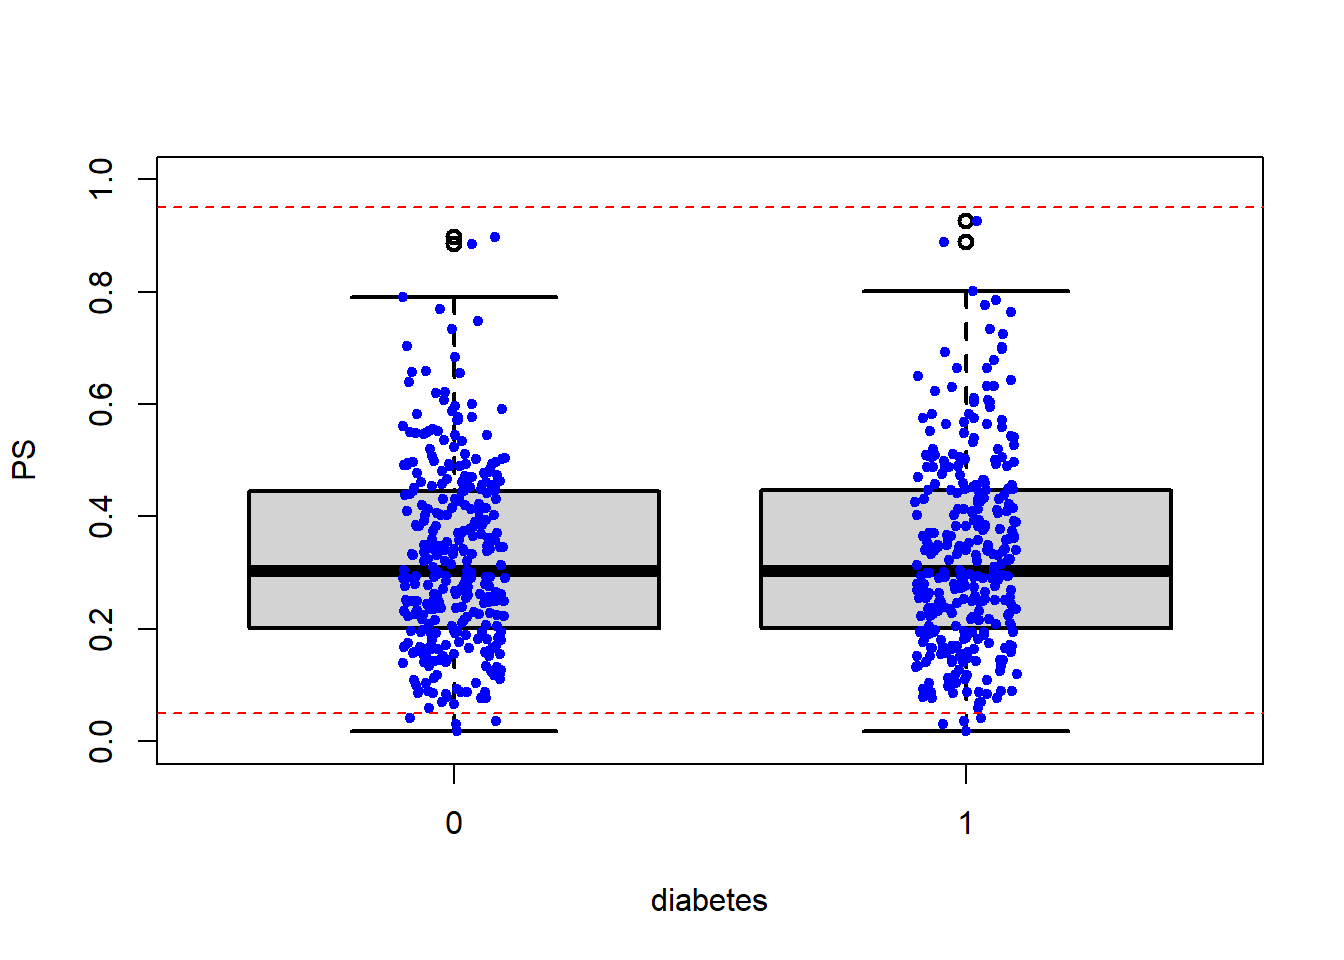
\includegraphics[width=0.3\linewidth]{UnderstandingPropensityScore_files/figure-latex/ps3cgvv-1}

\begin{itemize}
\tightlist
\item
  Sensitivity analysis should be done with trimming.
\item
  Have consequences in interpretation

  \begin{itemize}
  \tightlist
  \item
    target populstion may be unclear
  \end{itemize}
\end{itemize}

\hypertarget{unsatirfactory-balance}{%
\section{Unsatirfactory balance}\label{unsatirfactory-balance}}

\begin{itemize}
\tightlist
\item
  Best strategy is to go back to step 2, and make changes in the PS model specification
\end{itemize}

\hypertarget{s4}{%
\chapter{Step 4: Outcome modelling}\label{s4}}

\begin{itemize}
\tightlist
\item
  Some flexibility in choosing outcome model

  \begin{itemize}
  \tightlist
  \item
    considered independent of exposure modelling
  \item
    some propose double robust approach
  \item
    adjusting imbalanced covariates only?

    \begin{itemize}
    \tightlist
    \item
      double-adjustment may address residual confounding \citep{nguyen2017double}
    \end{itemize}
  \end{itemize}
\end{itemize}

\hypertarget{crude-outcome-model}{%
\section{Crude outcome model}\label{crude-outcome-model}}

Estimate the effect of treatment on outcomes using propensity score-matched sample

\begin{Shaded}
\begin{Highlighting}[]
\NormalTok{fit3 }\OtherTok{\textless{}{-}} \FunctionTok{glm}\NormalTok{(cholesterol}\SpecialCharTok{\textasciitilde{}}\NormalTok{diabetes,}
            \AttributeTok{family=}\NormalTok{binomial, }\AttributeTok{data =}\NormalTok{ matched.data)}
\FunctionTok{publish}\NormalTok{(fit3)}
\end{Highlighting}
\end{Shaded}

\begin{verbatim}
##  Variable Units OddsRatio       CI.95  p-value 
##  diabetes            0.90 [0.54;1.50]   0.6984
\end{verbatim}

\hypertarget{double-adjustment}{%
\section{Double-adjustment}\label{double-adjustment}}

Estimate the effect of treatment on outcomes using propensity score-matched sample, and adjust for imbalanced covariate

\begin{Shaded}
\begin{Highlighting}[]
\NormalTok{fit3r }\OtherTok{\textless{}{-}} \FunctionTok{glm}\NormalTok{(cholesterol}\SpecialCharTok{\textasciitilde{}}\NormalTok{diabetes }\SpecialCharTok{+}\NormalTok{ race,}
            \AttributeTok{family=}\NormalTok{binomial, }\AttributeTok{data =}\NormalTok{ matched.data)}
\FunctionTok{publish}\NormalTok{(fit3r)}
\end{Highlighting}
\end{Shaded}

\begin{verbatim}
##  Variable    Units OddsRatio       CI.95  p-value 
##  diabetes               0.89 [0.54;1.49]   0.6657 
##      race    Black       Ref                      
##           Hispanic      0.96 [0.46;2.02]   0.9165 
##              Other      1.32 [0.63;2.78]   0.4581 
##              White      0.58 [0.30;1.13]   0.1095
\end{verbatim}

\hypertarget{adjusted-outcome-model}{%
\section{Adjusted outcome model}\label{adjusted-outcome-model}}

Adjust for all covariates, again! (suggested)

\begin{Shaded}
\begin{Highlighting}[]
\NormalTok{out.formula }\OtherTok{\textless{}{-}} \FunctionTok{as.formula}\NormalTok{(}\FunctionTok{paste}\NormalTok{(}\StringTok{"cholesterol"}\NormalTok{, }\StringTok{"\textasciitilde{} diabetes +"}\NormalTok{, }
                               \FunctionTok{paste}\NormalTok{(baselinevars, }
                                     \AttributeTok{collapse =} \StringTok{"+"}\NormalTok{)))}
\NormalTok{out.formula}
\end{Highlighting}
\end{Shaded}

\begin{verbatim}
## cholesterol ~ diabetes + gender + age + race + education + married + 
##     bmi
\end{verbatim}

\begin{Shaded}
\begin{Highlighting}[]
\NormalTok{fit3b }\OtherTok{\textless{}{-}} \FunctionTok{glm}\NormalTok{(out.formula,}
            \AttributeTok{family=}\NormalTok{binomial, }\AttributeTok{data =}\NormalTok{ matched.data)}
\FunctionTok{publish}\NormalTok{(fit3b)}
\end{Highlighting}
\end{Shaded}

\begin{verbatim}
##   Variable              Units OddsRatio       CI.95     p-value 
##   diabetes                         0.86 [0.51;1.46]   0.5794126 
##     gender             Female       Ref                         
##                          Male      0.38 [0.21;0.69]   0.0012767 
##        age                         0.95 [0.93;0.97]     < 1e-04 
##       race              Black       Ref                         
##                      Hispanic      0.72 [0.31;1.65]   0.4346787 
##                         Other      0.77 [0.34;1.73]   0.5224157 
##                         White      0.51 [0.25;1.04]   0.0649791 
##  education            College       Ref                         
##                   High.School      0.70 [0.39;1.24]   0.2215142 
##                        School      0.93 [0.35;2.43]   0.8791455 
##    married            Married       Ref                         
##                 Never.married      0.48 [0.15;1.54]   0.2173180 
##            Previously.married      0.84 [0.45;1.57]   0.5900732 
##        bmi                         0.93 [0.89;0.97]   0.0005547
\end{verbatim}

The above analysis do not take matched pair into consideration while regressing.

\hypertarget{other-cosiderations-for-outcome-model}{%
\section{Other cosiderations for outcome model}\label{other-cosiderations-for-outcome-model}}

Literature proposes different strategies:

\begin{itemize}
\tightlist
\item
  do not control for pairs / clusters

  \begin{itemize}
  \tightlist
  \item
    use \texttt{glm} as is
  \end{itemize}
\item
  control for pairs / clusters

  \begin{itemize}
  \tightlist
  \item
    use \texttt{cluster} option (preferred)
  \item
    use GEE or
  \item
    use conditional logistic
  \end{itemize}
\end{itemize}

Here is an example using cluster option:

\begin{Shaded}
\begin{Highlighting}[]
\FunctionTok{require}\NormalTok{(jtools)}
\FunctionTok{summ}\NormalTok{(fit3b, }\AttributeTok{rubust =} \StringTok{"HC0"}\NormalTok{, }\AttributeTok{confint =} \ConstantTok{TRUE}\NormalTok{, }\AttributeTok{digists =} \DecValTok{3}\NormalTok{, }
     \AttributeTok{cluster =} \StringTok{"subclass"}\NormalTok{, }\AttributeTok{model.info =} \ConstantTok{FALSE}\NormalTok{, }
     \AttributeTok{model.fit =} \ConstantTok{FALSE}\NormalTok{, }\AttributeTok{exp =} \ConstantTok{TRUE}\NormalTok{)}
\end{Highlighting}
\end{Shaded}

\begin{table}[!h]
\centering
\begin{threeparttable}
\begin{tabular}{lrrrrr}
\toprule
  & exp(Est.) & 2.5\% & 97.5\% & z val. & p\\
\midrule
\cellcolor{gray!6}{(Intercept)} & \cellcolor{gray!6}{100.02} & \cellcolor{gray!6}{8.74} & \cellcolor{gray!6}{1144.55} & \cellcolor{gray!6}{3.70} & \cellcolor{gray!6}{0.00}\\
diabetes & 0.86 & 0.51 & 1.46 & -0.55 & 0.58\\
\cellcolor{gray!6}{genderMale} & \cellcolor{gray!6}{0.38} & \cellcolor{gray!6}{0.21} & \cellcolor{gray!6}{0.69} & \cellcolor{gray!6}{-3.22} & \cellcolor{gray!6}{0.00}\\
age & 0.95 & 0.93 & 0.97 & -4.47 & 0.00\\
\cellcolor{gray!6}{raceHispanic} & \cellcolor{gray!6}{0.72} & \cellcolor{gray!6}{0.31} & \cellcolor{gray!6}{1.65} & \cellcolor{gray!6}{-0.78} & \cellcolor{gray!6}{0.43}\\
\addlinespace
raceOther & 0.77 & 0.34 & 1.73 & -0.64 & 0.52\\
\cellcolor{gray!6}{raceWhite} & \cellcolor{gray!6}{0.51} & \cellcolor{gray!6}{0.25} & \cellcolor{gray!6}{1.04} & \cellcolor{gray!6}{-1.85} & \cellcolor{gray!6}{0.06}\\
educationHigh.School & 0.70 & 0.39 & 1.24 & -1.22 & 0.22\\
\cellcolor{gray!6}{educationSchool} & \cellcolor{gray!6}{0.93} & \cellcolor{gray!6}{0.35} & \cellcolor{gray!6}{2.43} & \cellcolor{gray!6}{-0.15} & \cellcolor{gray!6}{0.88}\\
marriedNever.married & 0.48 & 0.15 & 1.54 & -1.23 & 0.22\\
\addlinespace
\cellcolor{gray!6}{marriedPreviously.married} & \cellcolor{gray!6}{0.84} & \cellcolor{gray!6}{0.45} & \cellcolor{gray!6}{1.57} & \cellcolor{gray!6}{-0.54} & \cellcolor{gray!6}{0.59}\\
bmi & 0.93 & 0.89 & 0.97 & -3.45 & 0.00\\
\bottomrule
\end{tabular}
\begin{tablenotes}
\item Standard errors: MLE
\end{tablenotes}
\end{threeparttable}
\end{table}

\begin{itemize}
\tightlist
\item
  Bootstrap for matched pairfor WOR \citep{austin2014use}

  \begin{itemize}
  \tightlist
  \item
    may not be appropriate for WR
  \end{itemize}
\end{itemize}

\hypertarget{estimate-obtained}{%
\section{Estimate obtained}\label{estimate-obtained}}

\begin{itemize}
\tightlist
\item
  The example compared \texttt{diabetic} (a treated group; target) vs \texttt{Not\ diabetic} (untreated).
\item
  Thc corresponding treatment effect estimate is known as

  \begin{itemize}
  \tightlist
  \item
    Average Treatment Effects on the Treated (\textbf{ATT})
  \end{itemize}
\item
  Other estimates from PS analysis (e.g., PS weighting) are possible that compared the whole population

  \begin{itemize}
  \tightlist
  \item
    what if everyone treated vs.~what if nobody was treated (ATE)
  \end{itemize}
\end{itemize}

\hypertarget{compare}{%
\chapter{PS vs.~Regression}\label{compare}}

\hypertarget{data-simulation}{%
\section{Data Simulation}\label{data-simulation}}

Simplified simulation example, so that we know the true parameter \(\theta\).

\begin{longtable}[]{@{}ll@{}}
\toprule
\endhead
\(Y\) : Outcome & Cholesterol levels (continuous)\tabularnewline
\(A\) : Exposure & Diabetes\tabularnewline
\(L\) : Known Confounders & age (continuous)\tabularnewline
\bottomrule
\end{longtable}

\begin{itemize}
\tightlist
\item
  Confounder \(L\) (continuous)

  \begin{itemize}
  \tightlist
  \item
    Logit \(L\) \textasciitilde{} N(mean = 10, sd = 1)
  \end{itemize}
\item
  Treatment \(A\) (binary 0/1)

  \begin{itemize}
  \tightlist
  \item
    Logit \(P(A = 1)\) \textasciitilde{} 0.4 L
  \end{itemize}
\item
  Outcome \(Y\) (continuous)

  \begin{itemize}
  \tightlist
  \item
    Y \textasciitilde{} N(mean = 3 L + \(\theta\) A, sd = 1)
  \end{itemize}
\end{itemize}

\(\theta = 0.7\)

\begin{Shaded}
\begin{Highlighting}[]
\FunctionTok{require}\NormalTok{(simcausal)}
\NormalTok{D }\OtherTok{\textless{}{-}} \FunctionTok{DAG.empty}\NormalTok{()}
\NormalTok{D }\OtherTok{\textless{}{-}}\NormalTok{ D }\SpecialCharTok{+}
  \FunctionTok{node}\NormalTok{(}\StringTok{"L"}\NormalTok{, }\AttributeTok{distr =} \StringTok{"rnorm"}\NormalTok{, }\AttributeTok{mean =} \DecValTok{10}\NormalTok{, }\AttributeTok{sd =} \DecValTok{1}\NormalTok{) }\SpecialCharTok{+}
  \FunctionTok{node}\NormalTok{(}\StringTok{"A"}\NormalTok{, }\AttributeTok{distr =} \StringTok{"rbern"}\NormalTok{, }\AttributeTok{prob =} \FunctionTok{plogis}\NormalTok{(}\FloatTok{0.4}\SpecialCharTok{*}\NormalTok{L)) }\SpecialCharTok{+}
  \FunctionTok{node}\NormalTok{(}\StringTok{"Y"}\NormalTok{, }\AttributeTok{distr =} \StringTok{"rnorm"}\NormalTok{, }\AttributeTok{mean =} \DecValTok{3} \SpecialCharTok{*}\NormalTok{ L }\SpecialCharTok{+} \FloatTok{0.7} \SpecialCharTok{*}\NormalTok{ A, }\AttributeTok{sd =} \DecValTok{1}\NormalTok{)}
\NormalTok{Dset }\OtherTok{\textless{}{-}} \FunctionTok{set.DAG}\NormalTok{(D)}
\end{Highlighting}
\end{Shaded}

\begin{Shaded}
\begin{Highlighting}[]
\FunctionTok{plotDAG}\NormalTok{(Dset, }\AttributeTok{xjitter =} \FloatTok{0.1}\NormalTok{, }\AttributeTok{yjitter =}\NormalTok{ .}\DecValTok{9}\NormalTok{,}
        \AttributeTok{edge\_attrs =} \FunctionTok{list}\NormalTok{(}\AttributeTok{width =} \FloatTok{0.5}\NormalTok{, }\AttributeTok{arrow.width =} \FloatTok{0.4}\NormalTok{, }\AttributeTok{arrow.size =} \FloatTok{1.7}\NormalTok{),}
        \AttributeTok{vertex\_attrs =} \FunctionTok{list}\NormalTok{(}\AttributeTok{size =} \DecValTok{18}\NormalTok{, }\AttributeTok{label.cex =} \FloatTok{1.8}\NormalTok{))}
\end{Highlighting}
\end{Shaded}

\begin{verbatim}
## using the following vertex attributes:
\end{verbatim}

\begin{verbatim}
## 181.8NAdarkbluenone0
\end{verbatim}

\begin{verbatim}
## using the following edge attributes:
\end{verbatim}

\begin{verbatim}
## 0.50.41.7black1
\end{verbatim}

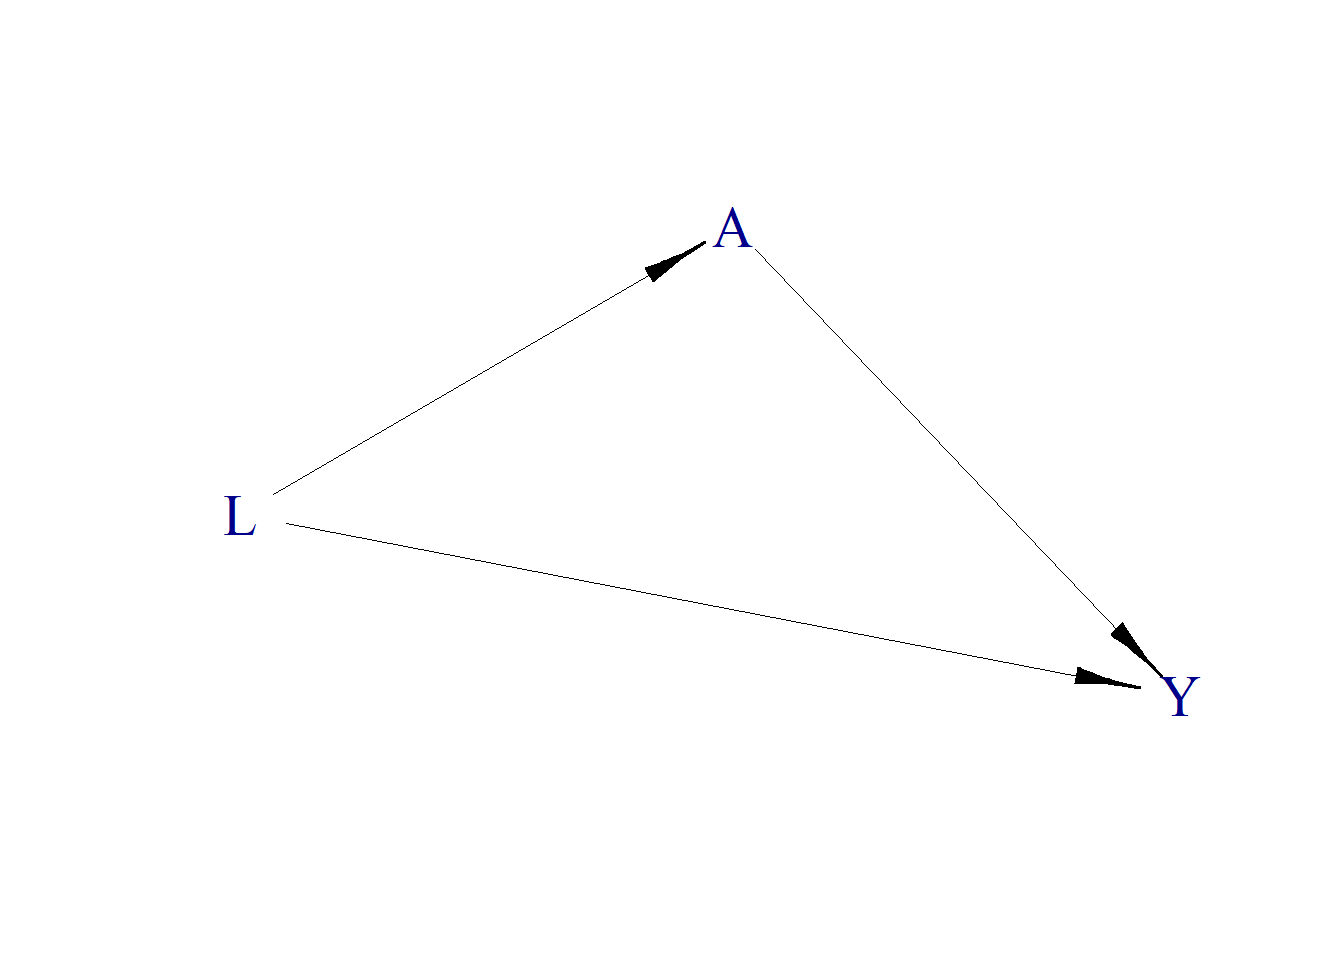
\includegraphics{UnderstandingPropensityScore_files/figure-latex/unnamed-chunk-25-1.pdf}

\begin{Shaded}
\begin{Highlighting}[]
\CommentTok{\# Data generating function}
\NormalTok{fnc }\OtherTok{\textless{}{-}} \ControlFlowTok{function}\NormalTok{(}\AttributeTok{n =} \DecValTok{10}\NormalTok{, }\AttributeTok{seedx =} \DecValTok{123}\NormalTok{)\{}
  \FunctionTok{require}\NormalTok{(simcausal)}
  \FunctionTok{set.seed}\NormalTok{(seedx)}
\NormalTok{  D }\OtherTok{\textless{}{-}} \FunctionTok{DAG.empty}\NormalTok{()}
\NormalTok{  D }\OtherTok{\textless{}{-}}\NormalTok{ D }\SpecialCharTok{+}
    \FunctionTok{node}\NormalTok{(}\StringTok{"L"}\NormalTok{, }\AttributeTok{distr =} \StringTok{"rnorm"}\NormalTok{, }\AttributeTok{mean =} \DecValTok{10}\NormalTok{, }\AttributeTok{sd =} \DecValTok{1}\NormalTok{) }\SpecialCharTok{+}
    \FunctionTok{node}\NormalTok{(}\StringTok{"A"}\NormalTok{, }\AttributeTok{distr =} \StringTok{"rbern"}\NormalTok{, }\AttributeTok{prob =} \FunctionTok{plogis}\NormalTok{(}\FloatTok{0.4}\SpecialCharTok{*}\NormalTok{L)) }\SpecialCharTok{+}
    \FunctionTok{node}\NormalTok{(}\StringTok{"Y"}\NormalTok{, }\AttributeTok{distr =} \StringTok{"rnorm"}\NormalTok{, }\AttributeTok{mean =} \DecValTok{3} \SpecialCharTok{*}\NormalTok{ L }\SpecialCharTok{+} \FloatTok{0.7} \SpecialCharTok{*}\NormalTok{ A, }\AttributeTok{sd =} \DecValTok{1}\NormalTok{)}
\NormalTok{  Dset }\OtherTok{\textless{}{-}} \FunctionTok{set.DAG}\NormalTok{(D)}
\NormalTok{  A1 }\OtherTok{\textless{}{-}} \FunctionTok{node}\NormalTok{(}\StringTok{"A"}\NormalTok{, }\AttributeTok{distr =} \StringTok{"rbern"}\NormalTok{, }\AttributeTok{prob =} \DecValTok{1}\NormalTok{)}
\NormalTok{  Dset }\OtherTok{\textless{}{-}}\NormalTok{ Dset }\SpecialCharTok{+} \FunctionTok{action}\NormalTok{(}\StringTok{"A1"}\NormalTok{, }\AttributeTok{nodes =}\NormalTok{ A1)}
\NormalTok{  A0 }\OtherTok{\textless{}{-}} \FunctionTok{node}\NormalTok{(}\StringTok{"A"}\NormalTok{, }\AttributeTok{distr =} \StringTok{"rbern"}\NormalTok{, }\AttributeTok{prob =} \DecValTok{0}\NormalTok{)}
\NormalTok{  Dset }\OtherTok{\textless{}{-}}\NormalTok{ Dset }\SpecialCharTok{+} \FunctionTok{action}\NormalTok{(}\StringTok{"A0"}\NormalTok{, }\AttributeTok{nodes =}\NormalTok{ A0)}
\NormalTok{  Cdat }\OtherTok{\textless{}{-}} \FunctionTok{sim}\NormalTok{(}\AttributeTok{DAG =}\NormalTok{ Dset, }\AttributeTok{actions =} \FunctionTok{c}\NormalTok{(}\StringTok{"A1"}\NormalTok{, }\StringTok{"A0"}\NormalTok{), }\AttributeTok{n =}\NormalTok{ n, }\AttributeTok{rndseed =} \DecValTok{123}\NormalTok{)}
\NormalTok{  generated.data }\OtherTok{\textless{}{-}} \FunctionTok{round}\NormalTok{(}\FunctionTok{cbind}\NormalTok{(Cdat}\SpecialCharTok{$}\NormalTok{A1[}\FunctionTok{c}\NormalTok{(}\StringTok{"ID"}\NormalTok{, }\StringTok{"L"}\NormalTok{, }\StringTok{"Y"}\NormalTok{)],Cdat}\SpecialCharTok{$}\NormalTok{A0[}\FunctionTok{c}\NormalTok{(}\StringTok{"Y"}\NormalTok{)]),}\DecValTok{2}\NormalTok{)}
  \FunctionTok{names}\NormalTok{(generated.data) }\OtherTok{\textless{}{-}} \FunctionTok{c}\NormalTok{(}\StringTok{"ID"}\NormalTok{, }\StringTok{"L"}\NormalTok{, }\StringTok{"Y1"}\NormalTok{, }\StringTok{"Y0"}\NormalTok{)}
\NormalTok{  generated.data }\OtherTok{\textless{}{-}}\NormalTok{ generated.data[}\FunctionTok{order}\NormalTok{(generated.data}\SpecialCharTok{$}\NormalTok{L, generated.data}\SpecialCharTok{$}\NormalTok{ID),]}
\NormalTok{  generated.data}\SpecialCharTok{$}\NormalTok{A }\OtherTok{\textless{}{-}} \FunctionTok{sample}\NormalTok{(}\FunctionTok{c}\NormalTok{(}\DecValTok{0}\NormalTok{,}\DecValTok{1}\NormalTok{),n, }\AttributeTok{replace =} \ConstantTok{TRUE}\NormalTok{)}
\NormalTok{  generated.data}\SpecialCharTok{$}\NormalTok{Y }\OtherTok{\textless{}{-}} \FunctionTok{ifelse}\NormalTok{(generated.data}\SpecialCharTok{$}\NormalTok{A}\SpecialCharTok{==}\DecValTok{0}\NormalTok{, generated.data}\SpecialCharTok{$}\NormalTok{Y0, generated.data}\SpecialCharTok{$}\NormalTok{Y1)}
\NormalTok{  counterfactual.dataset}\OtherTok{\textless{}{-}}\NormalTok{ generated.data[}\FunctionTok{order}\NormalTok{(generated.data}\SpecialCharTok{$}\NormalTok{ID) , ][}\FunctionTok{c}\NormalTok{(}\StringTok{"ID"}\NormalTok{,}\StringTok{"L"}\NormalTok{,}\StringTok{"A"}\NormalTok{,}\StringTok{"Y1"}\NormalTok{,}\StringTok{"Y0"}\NormalTok{)]}
\NormalTok{  observed.dataset}\OtherTok{\textless{}{-}}\NormalTok{ generated.data[}\FunctionTok{order}\NormalTok{(generated.data}\SpecialCharTok{$}\NormalTok{ID) , ][}\FunctionTok{c}\NormalTok{(}\StringTok{"ID"}\NormalTok{,}\StringTok{"L"}\NormalTok{,}\StringTok{"A"}\NormalTok{,}\StringTok{"Y"}\NormalTok{)]}
  \FunctionTok{return}\NormalTok{(}\FunctionTok{list}\NormalTok{(}\AttributeTok{counterfactual=}\NormalTok{counterfactual.dataset,}
              \AttributeTok{observed=}\NormalTok{observed.dataset))}
\NormalTok{\}}
\end{Highlighting}
\end{Shaded}

10 observations from the data generation:

\begin{Shaded}
\begin{Highlighting}[]
\NormalTok{result.data }\OtherTok{\textless{}{-}} \FunctionTok{fnc}\NormalTok{(}\AttributeTok{n=}\DecValTok{10}\NormalTok{)  }
\end{Highlighting}
\end{Shaded}

\begin{Shaded}
\begin{Highlighting}[]
\NormalTok{result.data}
\end{Highlighting}
\end{Shaded}

\begin{verbatim}
## $counterfactual
##    ID     L A    Y1    Y0
## 1   1  9.44 0 30.24 29.54
## 2   2  9.77 1 30.37 29.67
## 3   3 11.56 1 35.78 35.08
## 4   4 10.07 0 31.02 30.32
## 5   5 10.13 0 30.53 29.83
## 6   6 11.72 0 37.63 36.93
## 7   7 10.46 1 32.58 31.88
## 8   8  8.73 1 24.94 24.24
## 9   9  9.31 1 29.34 28.64
## 10 10  9.55 1 28.89 28.19
## 
## $observed
##    ID     L A     Y
## 1   1  9.44 0 29.54
## 2   2  9.77 1 30.37
## 3   3 11.56 1 35.78
## 4   4 10.07 0 30.32
## 5   5 10.13 0 29.83
## 6   6 11.72 0 36.93
## 7   7 10.46 1 32.58
## 8   8  8.73 1 24.94
## 9   9  9.31 1 29.34
## 10 10  9.55 1 28.89
\end{verbatim}

\hypertarget{treatment-effect-from-counterfactuals}{%
\section{Treatment effect from counterfactuals}\label{treatment-effect-from-counterfactuals}}

True \(\theta\) can be obtained from counterfactual data:

\begin{Shaded}
\begin{Highlighting}[]
\NormalTok{result.data}\SpecialCharTok{$}\NormalTok{counterfactual}\SpecialCharTok{$}\NormalTok{TE }\OtherTok{\textless{}{-}}\NormalTok{ result.data}\SpecialCharTok{$}\NormalTok{counterfactual}\SpecialCharTok{$}\NormalTok{Y1}\SpecialCharTok{{-}}\NormalTok{ result.data}\SpecialCharTok{$}\NormalTok{counterfactual}\SpecialCharTok{$}\NormalTok{Y0}
\NormalTok{result.data}\SpecialCharTok{$}\NormalTok{counterfactual}
\end{Highlighting}
\end{Shaded}

\begin{verbatim}
##    ID     L A    Y1    Y0  TE
## 1   1  9.44 0 30.24 29.54 0.7
## 2   2  9.77 1 30.37 29.67 0.7
## 3   3 11.56 1 35.78 35.08 0.7
## 4   4 10.07 0 31.02 30.32 0.7
## 5   5 10.13 0 30.53 29.83 0.7
## 6   6 11.72 0 37.63 36.93 0.7
## 7   7 10.46 1 32.58 31.88 0.7
## 8   8  8.73 1 24.94 24.24 0.7
## 9   9  9.31 1 29.34 28.64 0.7
## 10 10  9.55 1 28.89 28.19 0.7
\end{verbatim}

\hypertarget{treatment-effect-from-regression}{%
\section{Treatment effect from Regression}\label{treatment-effect-from-regression}}

What happens in observed data for a sample of size 10?

\begin{Shaded}
\begin{Highlighting}[]
\FunctionTok{round}\NormalTok{(}\FunctionTok{coef}\NormalTok{(}\FunctionTok{glm}\NormalTok{(Y }\SpecialCharTok{\textasciitilde{}}\NormalTok{ A, }\AttributeTok{family=}\StringTok{"gaussian"}\NormalTok{, }\AttributeTok{data=}\NormalTok{result.data}\SpecialCharTok{$}\NormalTok{observed)),}\DecValTok{2}\NormalTok{)}
\end{Highlighting}
\end{Shaded}

\begin{verbatim}
## (Intercept)           A 
##       31.65       -1.34
\end{verbatim}

\begin{Shaded}
\begin{Highlighting}[]
\FunctionTok{round}\NormalTok{(}\FunctionTok{coef}\NormalTok{(}\FunctionTok{glm}\NormalTok{(Y }\SpecialCharTok{\textasciitilde{}}\NormalTok{ A }\SpecialCharTok{+}\NormalTok{ L, }\AttributeTok{family=}\StringTok{"gaussian"}\NormalTok{, }\AttributeTok{data=}\NormalTok{result.data}\SpecialCharTok{$}\NormalTok{observed)),}\DecValTok{2}\NormalTok{)}
\end{Highlighting}
\end{Shaded}

\begin{verbatim}
## (Intercept)           A           L 
##       -5.17        0.24        3.56
\end{verbatim}

What happens in observed data for a sample of size 10000?

\begin{Shaded}
\begin{Highlighting}[]
\NormalTok{result.data }\OtherTok{\textless{}{-}} \FunctionTok{fnc}\NormalTok{(}\AttributeTok{n=}\DecValTok{10000}\NormalTok{)}
\end{Highlighting}
\end{Shaded}

\begin{Shaded}
\begin{Highlighting}[]
\FunctionTok{round}\NormalTok{(}\FunctionTok{coef}\NormalTok{(}\FunctionTok{glm}\NormalTok{(Y }\SpecialCharTok{\textasciitilde{}}\NormalTok{ A, }\AttributeTok{family=}\StringTok{"gaussian"}\NormalTok{, }\AttributeTok{data=}\NormalTok{result.data}\SpecialCharTok{$}\NormalTok{observed)),}\DecValTok{2}\NormalTok{)}
\end{Highlighting}
\end{Shaded}

\begin{verbatim}
## (Intercept)           A 
##       29.98        0.70
\end{verbatim}

\begin{Shaded}
\begin{Highlighting}[]
\FunctionTok{round}\NormalTok{(}\FunctionTok{coef}\NormalTok{(}\FunctionTok{glm}\NormalTok{(Y }\SpecialCharTok{\textasciitilde{}}\NormalTok{ A }\SpecialCharTok{+}\NormalTok{ L, }\AttributeTok{family=}\StringTok{"gaussian"}\NormalTok{, }\AttributeTok{data=}\NormalTok{result.data}\SpecialCharTok{$}\NormalTok{observed)),}\DecValTok{2}\NormalTok{)}
\end{Highlighting}
\end{Shaded}

\begin{verbatim}
## (Intercept)           A           L 
##       -0.07        0.70        3.01
\end{verbatim}

\hypertarget{treatment-effect-from-ps}{%
\section{Treatment effect from PS}\label{treatment-effect-from-ps}}

Propensity score model fitting:

\begin{Shaded}
\begin{Highlighting}[]
\FunctionTok{require}\NormalTok{(MatchIt)}
\NormalTok{match.obj }\OtherTok{\textless{}{-}} \FunctionTok{matchit}\NormalTok{(A }\SpecialCharTok{\textasciitilde{}}\NormalTok{ L, }\AttributeTok{method =} \StringTok{"nearest"}\NormalTok{, }
                     \AttributeTok{data =}\NormalTok{ result.data}\SpecialCharTok{$}\NormalTok{observed,}
                     \AttributeTok{distance =} \StringTok{\textquotesingle{}logit\textquotesingle{}}\NormalTok{, }
                     \AttributeTok{caliper =} \FloatTok{0.001}\NormalTok{,}
                     \AttributeTok{replace =} \ConstantTok{FALSE}\NormalTok{, }
                     \AttributeTok{ratio =} \DecValTok{1}\NormalTok{)}
\NormalTok{match.obj}
\end{Highlighting}
\end{Shaded}

\begin{verbatim}
## A matchit object
##  - method: 1:1 nearest neighbor matching without replacement
##  - distance: Propensity score [caliper]
##              - estimated with logistic regression
##  - caliper: <distance> (0)
##  - number of obs.: 10000 (original), 8306 (matched)
##  - target estimand: ATT
##  - covariates: L
\end{verbatim}

Results from step 4: crude

\begin{Shaded}
\begin{Highlighting}[]
\NormalTok{matched.data }\OtherTok{\textless{}{-}} \FunctionTok{match.data}\NormalTok{(match.obj)}
\end{Highlighting}
\end{Shaded}

Results from step 4: adjusted

\begin{Shaded}
\begin{Highlighting}[]
\FunctionTok{round}\NormalTok{(}\FunctionTok{coef}\NormalTok{(}\FunctionTok{glm}\NormalTok{(Y }\SpecialCharTok{\textasciitilde{}}\NormalTok{ A, }\AttributeTok{family=}\StringTok{"gaussian"}\NormalTok{, }\AttributeTok{data=}\NormalTok{matched.data)),}\DecValTok{2}\NormalTok{)}
\end{Highlighting}
\end{Shaded}

\begin{verbatim}
## (Intercept)           A 
##       29.97        0.69
\end{verbatim}

\begin{Shaded}
\begin{Highlighting}[]
\FunctionTok{round}\NormalTok{(}\FunctionTok{coef}\NormalTok{(}\FunctionTok{glm}\NormalTok{(Y }\SpecialCharTok{\textasciitilde{}}\NormalTok{ A}\SpecialCharTok{+}\NormalTok{L, }\AttributeTok{family=}\StringTok{"gaussian"}\NormalTok{, }\AttributeTok{data=}\NormalTok{matched.data)),}\DecValTok{2}\NormalTok{)}
\end{Highlighting}
\end{Shaded}

\begin{verbatim}
## (Intercept)           A           L 
##       -0.10        0.69        3.01
\end{verbatim}

\hypertarget{non-linear-model}{%
\section{Non-linear Model}\label{non-linear-model}}

\hypertarget{data-generation}{%
\subsection{Data generation}\label{data-generation}}

\begin{longtable}[]{@{}ll@{}}
\toprule
\endhead
\(Y\) : Outcome & Cholesterol levels (continuous)\tabularnewline
\(A\) : Exposure & Diabetes\tabularnewline
\(L\) : Known Confounders & age (continuous)\tabularnewline
\bottomrule
\end{longtable}

\begin{itemize}
\tightlist
\item
  Confounder \(L\) (continuous)

  \begin{itemize}
  \tightlist
  \item
    Logit \(L\) \textasciitilde{} N(mean = 10, sd = 1)
  \end{itemize}
\item
  Treatment \(A\) (binary 0/1)

  \begin{itemize}
  \tightlist
  \item
    Logit \(P(A = 1)\) \textasciitilde{} 0.4 L
  \end{itemize}
\item
  Outcome \(Y\) (continuous)

  \begin{itemize}
  \tightlist
  \item
    Y \textasciitilde{} N(mean = 3 \(L^3\) + \(\theta\) A, sd = 1)
  \end{itemize}
\end{itemize}

\emph{The only difference} is \(L^3\) instead of \(L\) in the outcome mode.

Again, \(\theta = 0.7\)

\begin{Shaded}
\begin{Highlighting}[]
\CommentTok{\# Data generating function}
\NormalTok{fnc2 }\OtherTok{\textless{}{-}} \ControlFlowTok{function}\NormalTok{(}\AttributeTok{n =} \DecValTok{10}\NormalTok{, }\AttributeTok{seedx =} \DecValTok{123}\NormalTok{)\{}
  \FunctionTok{require}\NormalTok{(simcausal)}
  \FunctionTok{set.seed}\NormalTok{(seedx)}
\NormalTok{  D }\OtherTok{\textless{}{-}} \FunctionTok{DAG.empty}\NormalTok{()}
\NormalTok{  D }\OtherTok{\textless{}{-}}\NormalTok{ D }\SpecialCharTok{+}
    \FunctionTok{node}\NormalTok{(}\StringTok{"L"}\NormalTok{, }\AttributeTok{distr =} \StringTok{"rnorm"}\NormalTok{, }\AttributeTok{mean =} \DecValTok{10}\NormalTok{, }\AttributeTok{sd =} \DecValTok{1}\NormalTok{) }\SpecialCharTok{+}
    \FunctionTok{node}\NormalTok{(}\StringTok{"A"}\NormalTok{, }\AttributeTok{distr =} \StringTok{"rbern"}\NormalTok{, }\AttributeTok{prob =} \FunctionTok{plogis}\NormalTok{(}\FloatTok{0.4}\SpecialCharTok{*}\NormalTok{L)) }\SpecialCharTok{+}
    \FunctionTok{node}\NormalTok{(}\StringTok{"Y"}\NormalTok{, }\AttributeTok{distr =} \StringTok{"rnorm"}\NormalTok{, }\AttributeTok{mean =} \DecValTok{3} \SpecialCharTok{*}\NormalTok{ L}\SpecialCharTok{\^{}}\DecValTok{3} \SpecialCharTok{+} \FloatTok{0.7} \SpecialCharTok{*}\NormalTok{ A, }\AttributeTok{sd =} \DecValTok{1}\NormalTok{)}
\NormalTok{  Dset }\OtherTok{\textless{}{-}} \FunctionTok{set.DAG}\NormalTok{(D)}
\NormalTok{  A1 }\OtherTok{\textless{}{-}} \FunctionTok{node}\NormalTok{(}\StringTok{"A"}\NormalTok{, }\AttributeTok{distr =} \StringTok{"rbern"}\NormalTok{, }\AttributeTok{prob =} \DecValTok{1}\NormalTok{)}
\NormalTok{  Dset }\OtherTok{\textless{}{-}}\NormalTok{ Dset }\SpecialCharTok{+} \FunctionTok{action}\NormalTok{(}\StringTok{"A1"}\NormalTok{, }\AttributeTok{nodes =}\NormalTok{ A1)}
\NormalTok{  A0 }\OtherTok{\textless{}{-}} \FunctionTok{node}\NormalTok{(}\StringTok{"A"}\NormalTok{, }\AttributeTok{distr =} \StringTok{"rbern"}\NormalTok{, }\AttributeTok{prob =} \DecValTok{0}\NormalTok{)}
\NormalTok{  Dset }\OtherTok{\textless{}{-}}\NormalTok{ Dset }\SpecialCharTok{+} \FunctionTok{action}\NormalTok{(}\StringTok{"A0"}\NormalTok{, }\AttributeTok{nodes =}\NormalTok{ A0)}
\NormalTok{  Cdat }\OtherTok{\textless{}{-}} \FunctionTok{sim}\NormalTok{(}\AttributeTok{DAG =}\NormalTok{ Dset, }\AttributeTok{actions =} \FunctionTok{c}\NormalTok{(}\StringTok{"A1"}\NormalTok{, }\StringTok{"A0"}\NormalTok{), }\AttributeTok{n =}\NormalTok{ n, }\AttributeTok{rndseed =} \DecValTok{123}\NormalTok{)}
\NormalTok{  generated.data }\OtherTok{\textless{}{-}} \FunctionTok{round}\NormalTok{(}\FunctionTok{cbind}\NormalTok{(Cdat}\SpecialCharTok{$}\NormalTok{A1[}\FunctionTok{c}\NormalTok{(}\StringTok{"ID"}\NormalTok{, }\StringTok{"L"}\NormalTok{, }\StringTok{"Y"}\NormalTok{)],Cdat}\SpecialCharTok{$}\NormalTok{A0[}\FunctionTok{c}\NormalTok{(}\StringTok{"Y"}\NormalTok{)]),}\DecValTok{2}\NormalTok{)}
  \FunctionTok{names}\NormalTok{(generated.data) }\OtherTok{\textless{}{-}} \FunctionTok{c}\NormalTok{(}\StringTok{"ID"}\NormalTok{, }\StringTok{"L"}\NormalTok{, }\StringTok{"Y1"}\NormalTok{, }\StringTok{"Y0"}\NormalTok{)}
\NormalTok{  generated.data }\OtherTok{\textless{}{-}}\NormalTok{ generated.data[}\FunctionTok{order}\NormalTok{(generated.data}\SpecialCharTok{$}\NormalTok{L, generated.data}\SpecialCharTok{$}\NormalTok{ID),]}
\NormalTok{  generated.data}\SpecialCharTok{$}\NormalTok{A }\OtherTok{\textless{}{-}} \FunctionTok{sample}\NormalTok{(}\FunctionTok{c}\NormalTok{(}\DecValTok{0}\NormalTok{,}\DecValTok{1}\NormalTok{),n, }\AttributeTok{replace =} \ConstantTok{TRUE}\NormalTok{)}
\NormalTok{  generated.data}\SpecialCharTok{$}\NormalTok{Y }\OtherTok{\textless{}{-}} \FunctionTok{ifelse}\NormalTok{(generated.data}\SpecialCharTok{$}\NormalTok{A}\SpecialCharTok{==}\DecValTok{0}\NormalTok{, generated.data}\SpecialCharTok{$}\NormalTok{Y0, generated.data}\SpecialCharTok{$}\NormalTok{Y1)}
\NormalTok{  counterfactual.dataset}\OtherTok{\textless{}{-}}\NormalTok{ generated.data[}\FunctionTok{order}\NormalTok{(generated.data}\SpecialCharTok{$}\NormalTok{ID) , ][}\FunctionTok{c}\NormalTok{(}\StringTok{"ID"}\NormalTok{,}\StringTok{"L"}\NormalTok{,}\StringTok{"A"}\NormalTok{,}\StringTok{"Y1"}\NormalTok{,}\StringTok{"Y0"}\NormalTok{)]}
\NormalTok{  observed.dataset}\OtherTok{\textless{}{-}}\NormalTok{ generated.data[}\FunctionTok{order}\NormalTok{(generated.data}\SpecialCharTok{$}\NormalTok{ID) , ][}\FunctionTok{c}\NormalTok{(}\StringTok{"ID"}\NormalTok{,}\StringTok{"L"}\NormalTok{,}\StringTok{"A"}\NormalTok{,}\StringTok{"Y"}\NormalTok{)]}
  \FunctionTok{return}\NormalTok{(}\FunctionTok{list}\NormalTok{(}\AttributeTok{counterfactual=}\NormalTok{counterfactual.dataset,}
              \AttributeTok{observed=}\NormalTok{observed.dataset))}
\NormalTok{\}}
\end{Highlighting}
\end{Shaded}

\hypertarget{regression}{%
\subsection{Regression}\label{regression}}

\begin{Shaded}
\begin{Highlighting}[]
\NormalTok{result.data }\OtherTok{\textless{}{-}} \FunctionTok{fnc2}\NormalTok{(}\AttributeTok{n=}\DecValTok{10000}\NormalTok{)}
\end{Highlighting}
\end{Shaded}

Crude estimates

\begin{Shaded}
\begin{Highlighting}[]
\FunctionTok{round}\NormalTok{(}\FunctionTok{coef}\NormalTok{(}\FunctionTok{glm}\NormalTok{(Y }\SpecialCharTok{\textasciitilde{}}\NormalTok{ A, }\AttributeTok{family=}\StringTok{"gaussian"}\NormalTok{, }\AttributeTok{data=}\NormalTok{result.data}\SpecialCharTok{$}\NormalTok{observed)),}\DecValTok{2}\NormalTok{)}
\end{Highlighting}
\end{Shaded}

\begin{verbatim}
## (Intercept)           A 
##     3094.49      -13.16
\end{verbatim}

Adjusted estimates

\begin{Shaded}
\begin{Highlighting}[]
\NormalTok{fit }\OtherTok{\textless{}{-}} \FunctionTok{glm}\NormalTok{(Y }\SpecialCharTok{\textasciitilde{}}\NormalTok{ A }\SpecialCharTok{+}\NormalTok{ L, }\AttributeTok{family=}\StringTok{"gaussian"}\NormalTok{, }\AttributeTok{data=}\NormalTok{result.data}\SpecialCharTok{$}\NormalTok{observed)}
\FunctionTok{round}\NormalTok{(}\FunctionTok{coef}\NormalTok{(fit),}\DecValTok{2}\NormalTok{)}
\end{Highlighting}
\end{Shaded}

\begin{verbatim}
## (Intercept)           A           L 
##    -6002.42       -1.25      909.32
\end{verbatim}

\begin{itemize}
\tightlist
\item
  In regression adjustments, the results could be subject to ``model extrapolation'' based on linearity assumption.

  \begin{itemize}
  \tightlist
  \item
    It is sometimes difficult to know whether the adjusted effect is based on extrapolation.
  \item
    Especially true in observational settings.
  \item
    PS may not need such linearity assumption (when non-parametric approaches used for prediction).

    \begin{itemize}
    \tightlist
    \item
      Don't necessarily mean non-parametric approaches are the best option though!
    \end{itemize}
  \end{itemize}
\end{itemize}

\hypertarget{ps-1}{%
\subsection{PS}\label{ps-1}}

Matching with PS

\begin{Shaded}
\begin{Highlighting}[]
\NormalTok{match.obj }\OtherTok{\textless{}{-}} \FunctionTok{matchit}\NormalTok{(A }\SpecialCharTok{\textasciitilde{}}\NormalTok{ L, }\AttributeTok{method =} \StringTok{"nearest"}\NormalTok{, }
                     \AttributeTok{data =}\NormalTok{ result.data}\SpecialCharTok{$}\NormalTok{observed,}
                     \AttributeTok{distance =} \StringTok{\textquotesingle{}logit\textquotesingle{}}\NormalTok{, }
                     \AttributeTok{replace =} \ConstantTok{FALSE}\NormalTok{, }
                     \AttributeTok{caliper =} \FloatTok{0.001}\NormalTok{,}
                     \AttributeTok{ratio =} \DecValTok{1}\NormalTok{)}
\NormalTok{match.obj}
\end{Highlighting}
\end{Shaded}

\begin{verbatim}
## A matchit object
##  - method: 1:1 nearest neighbor matching without replacement
##  - distance: Propensity score [caliper]
##              - estimated with logistic regression
##  - caliper: <distance> (0)
##  - number of obs.: 10000 (original), 8282 (matched)
##  - target estimand: ATT
##  - covariates: L
\end{verbatim}

\begin{Shaded}
\begin{Highlighting}[]
\NormalTok{matched.data }\OtherTok{\textless{}{-}} \FunctionTok{match.data}\NormalTok{(match.obj)}
\end{Highlighting}
\end{Shaded}

Results from step 4: crude

\begin{Shaded}
\begin{Highlighting}[]
\FunctionTok{round}\NormalTok{(}\FunctionTok{coef}\NormalTok{(}\FunctionTok{glm}\NormalTok{(Y }\SpecialCharTok{\textasciitilde{}}\NormalTok{ A, }\AttributeTok{family=}\StringTok{"gaussian"}\NormalTok{, }\AttributeTok{data=}\NormalTok{matched.data)),}\DecValTok{2}\NormalTok{)}
\end{Highlighting}
\end{Shaded}

\begin{verbatim}
## (Intercept)           A 
##     3070.64        0.72
\end{verbatim}

Results from step 4: adjusted

\begin{Shaded}
\begin{Highlighting}[]
\FunctionTok{round}\NormalTok{(}\FunctionTok{coef}\NormalTok{(}\FunctionTok{glm}\NormalTok{(Y }\SpecialCharTok{\textasciitilde{}}\NormalTok{ A}\SpecialCharTok{+}\NormalTok{L, }\AttributeTok{family=}\StringTok{"gaussian"}\NormalTok{, }\AttributeTok{data=}\NormalTok{matched.data)),}\DecValTok{2}\NormalTok{)}
\end{Highlighting}
\end{Shaded}

\begin{verbatim}
## (Intercept)           A           L 
##    -5980.08        0.72      905.62
\end{verbatim}

\hypertarget{machine-learning}{%
\subsection{Machine learning}\label{machine-learning}}

Using gradient boosted method for PS estimation

\begin{Shaded}
\begin{Highlighting}[]
\FunctionTok{require}\NormalTok{(twang)}
\NormalTok{result.data}\SpecialCharTok{$}\NormalTok{observed}\SpecialCharTok{$}\NormalTok{S }\OtherTok{\textless{}{-}} \DecValTok{0}
\NormalTok{ps.gbm }\OtherTok{\textless{}{-}} \FunctionTok{ps}\NormalTok{(A }\SpecialCharTok{\textasciitilde{}}\NormalTok{ L }\SpecialCharTok{+}\NormalTok{ S,}\AttributeTok{data =}\NormalTok{ result.data}\SpecialCharTok{$}\NormalTok{observed,}\AttributeTok{estimand =} \StringTok{"ATT"}\NormalTok{,}\AttributeTok{n.trees=}\DecValTok{1000}\NormalTok{)}
\FunctionTok{names}\NormalTok{(ps.gbm)}
\FunctionTok{summary}\NormalTok{(ps.gbm}\SpecialCharTok{$}\NormalTok{ps}\SpecialCharTok{$}\NormalTok{es.mean.ATT)}
\NormalTok{result.data}\SpecialCharTok{$}\NormalTok{observed}\SpecialCharTok{$}\NormalTok{ps }\OtherTok{\textless{}{-}}\NormalTok{ ps.gbm}\SpecialCharTok{$}\NormalTok{ps}\SpecialCharTok{$}\NormalTok{es.mean.ATT}
\end{Highlighting}
\end{Shaded}

Matching with PS generated from gradient boosted method

\begin{Shaded}
\begin{Highlighting}[]
\FunctionTok{require}\NormalTok{(Matching)}
\NormalTok{match.obj2 }\OtherTok{\textless{}{-}} \FunctionTok{Match}\NormalTok{(}\AttributeTok{Y=}\NormalTok{result.data}\SpecialCharTok{$}\NormalTok{observed}\SpecialCharTok{$}\NormalTok{Y, }\AttributeTok{Tr=}\NormalTok{result.data}\SpecialCharTok{$}\NormalTok{observed}\SpecialCharTok{$}\NormalTok{A, }
                    \AttributeTok{X=}\NormalTok{result.data}\SpecialCharTok{$}\NormalTok{observed}\SpecialCharTok{$}\NormalTok{ps, }\AttributeTok{M=}\DecValTok{1}\NormalTok{, }\AttributeTok{caliper =} \FloatTok{0.001}\NormalTok{,}
                    \AttributeTok{replace=}\ConstantTok{FALSE}\NormalTok{)}
\FunctionTok{summary}\NormalTok{(match.obj2)}
\end{Highlighting}
\end{Shaded}

\begin{verbatim}
## 
## Estimate...  1.5255 
## SE.........  1.6227 
## T-stat.....  0.94006 
## p.val......  0.34719 
## 
## Original number of observations..............  10000 
## Original number of treated obs...............  4968 
## Matched number of observations...............  4520 
## Matched number of observations  (unweighted).  4520 
## 
## Caliper (SDs)........................................   0.001 
## Number of obs dropped by 'exact' or 'caliper'  448
\end{verbatim}

\begin{Shaded}
\begin{Highlighting}[]
\NormalTok{matched.data2 }\OtherTok{\textless{}{-}}\NormalTok{ result.data}\SpecialCharTok{$}\NormalTok{observed[}\FunctionTok{c}\NormalTok{(match.obj2}\SpecialCharTok{$}\NormalTok{index.treated, match.obj2}\SpecialCharTok{$}\NormalTok{index.control),]}
\NormalTok{mb }\OtherTok{\textless{}{-}} \FunctionTok{MatchBalance}\NormalTok{(A}\SpecialCharTok{\textasciitilde{}}\NormalTok{L, }\AttributeTok{data=}\NormalTok{result.data}\SpecialCharTok{$}\NormalTok{observed, }\AttributeTok{match.out=}\NormalTok{match.obj2, }\AttributeTok{nboots=}\DecValTok{10}\NormalTok{)}
\end{Highlighting}
\end{Shaded}

Results from step 4: crude

\begin{Shaded}
\begin{Highlighting}[]
\FunctionTok{round}\NormalTok{(}\FunctionTok{coef}\NormalTok{(}\FunctionTok{glm}\NormalTok{(Y }\SpecialCharTok{\textasciitilde{}}\NormalTok{ A, }\AttributeTok{family=}\StringTok{"gaussian"}\NormalTok{, }\AttributeTok{data=}\NormalTok{matched.data2)),}\DecValTok{2}\NormalTok{)}
\end{Highlighting}
\end{Shaded}

\begin{verbatim}
## (Intercept)           A 
##     3089.17        1.53
\end{verbatim}

Results from step 4: adjusted

\begin{Shaded}
\begin{Highlighting}[]
\FunctionTok{round}\NormalTok{(}\FunctionTok{coef}\NormalTok{(}\FunctionTok{glm}\NormalTok{(Y }\SpecialCharTok{\textasciitilde{}}\NormalTok{ A}\SpecialCharTok{+}\NormalTok{L, }\AttributeTok{family=}\StringTok{"gaussian"}\NormalTok{, }\AttributeTok{data=}\NormalTok{matched.data2)),}\DecValTok{2}\NormalTok{)}
\end{Highlighting}
\end{Shaded}

\begin{verbatim}
## (Intercept)           A           L 
##    -6025.34        1.55      910.70
\end{verbatim}

\hypertarget{regression-is-doomed}{%
\subsection{Regression is doomed?}\label{regression-is-doomed}}

Not really. Always a god idea to check the diagnostic plots to find any indication of assumption violation:

\begin{Shaded}
\begin{Highlighting}[]
\FunctionTok{par}\NormalTok{(}\AttributeTok{mfrow=}\FunctionTok{c}\NormalTok{(}\DecValTok{2}\NormalTok{,}\DecValTok{2}\NormalTok{))}
\FunctionTok{plot}\NormalTok{(fit)}
\end{Highlighting}
\end{Shaded}

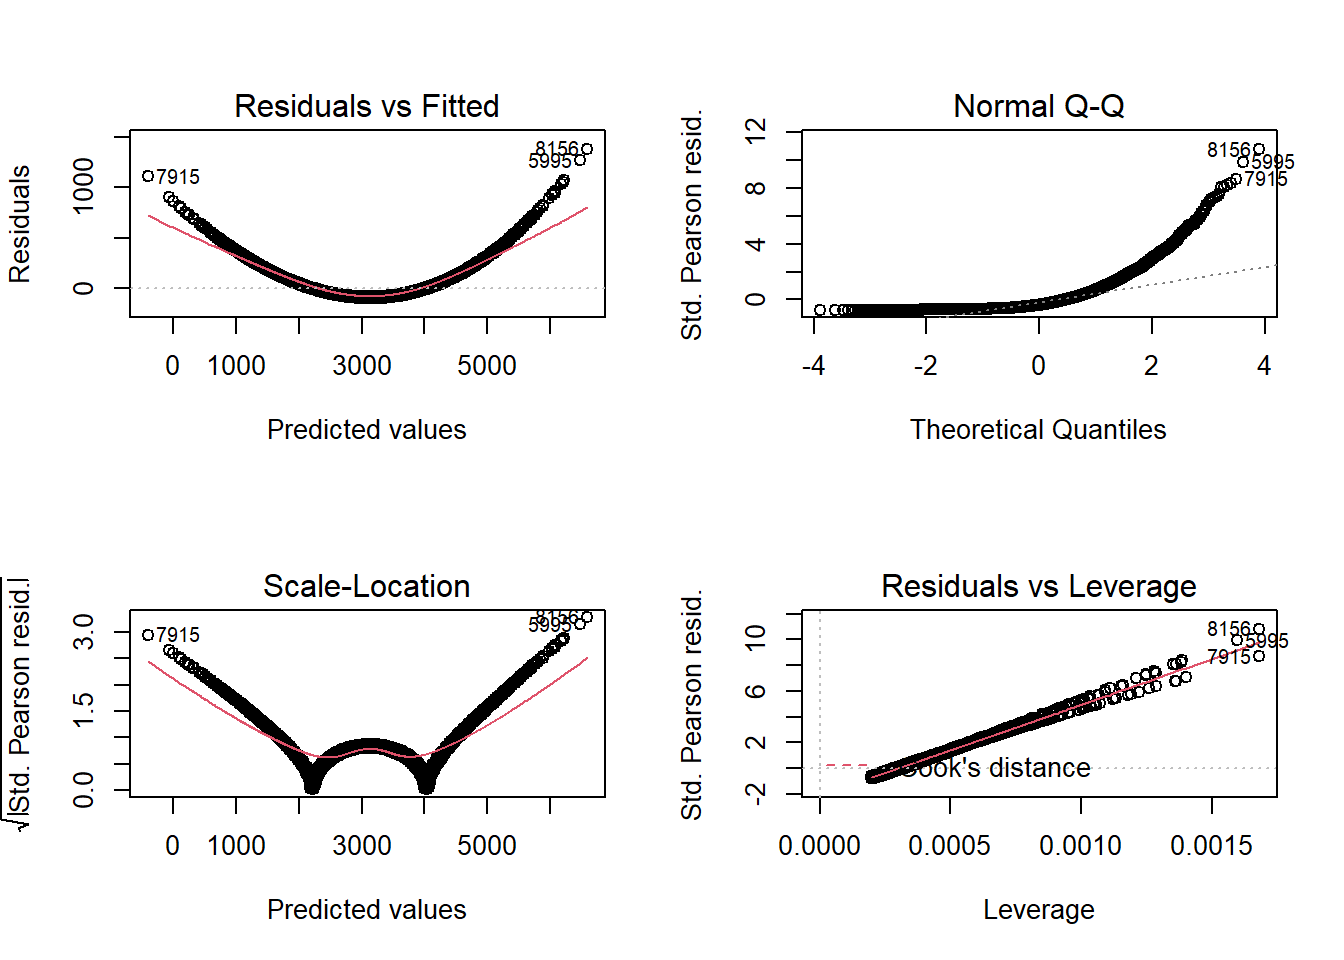
\includegraphics{UnderstandingPropensityScore_files/figure-latex/unnamed-chunk-48-1.pdf}

Residual plot has a pattern!

\begin{tabular}{l>{}l}
\toprule
![](images/info.png) & \cellcolor[HTML]{3A3B3C}{\textcolor{white}{Powerful machine learning method is good at prediction.}}\\
![](images/info.png) & \cellcolor[HTML]{3A3B3C}{\textcolor{white}{Propensity score methods rely on obtaining good balance.}}\\
![](images/info.png) & \cellcolor[HTML]{3A3B3C}{\textcolor{white}{Always a good idea to check analysis with multiple sensitivity analysis.}}\\
\bottomrule
\end{tabular}

\hypertarget{common-misconception}{%
\section{Common misconception}\label{common-misconception}}

\begin{itemize}
\tightlist
\item
  PS results = `causal';
\item
  regression = `non-causal'.
\end{itemize}

No.~`Results from both methods should lead to the same conclusions.' \citep{d1998propensity}

When the results deviate, important to investigate why!

\hypertarget{benifits-of-ps}{%
\section{Benifits of PS}\label{benifits-of-ps}}

\begin{itemize}
\item
  \textbf{Intuitive}: compare two similar groups
\item
  \textbf{2-step process}

  \begin{itemize}
  \tightlist
  \item
    Encourages researchers to think about the treatment generation process
  \item
    Fit outcome model with only important variables.
  \item
    Allowing to think more about design stage (nice separation from outcome model building process).
  \end{itemize}
\item
  Fit \textbf{rich PS model} (with higher order terms); focusing on prediction; worry less about overparameterization.

  \begin{itemize}
  \tightlist
  \item
    Non-parametric (ML) approaches can be used to relax linearity assumption in estimating PS.
  \item
    See more on \citet{lee2010improving}, \citet{pirracchio2015improving}, \citet{alam2019should}
  \end{itemize}
\item
  \textbf{Reduce dimension}, helpful when exposure frequent but outcome rare (event per variable).

  \begin{itemize}
  \tightlist
  \item
    Smaller outcome model may be helpful in diagnostic checks.
  \end{itemize}
\item
  \textbf{Diagnostics}

  \begin{itemize}
  \tightlist
  \item
    Diagnostics (balance checking) much easier compared to residual plot/influence
  \item
    Graphical comparison helps identify areas of non-overlap.
  \end{itemize}
\end{itemize}

\hypertarget{limitations-of-ps}{%
\section{Limitations of PS}\label{limitations-of-ps}}

\begin{itemize}
\tightlist
\item
  Matching population vs.~target population: often not the same.

  \begin{itemize}
  \tightlist
  \item
    PS matching may give effect estimate of a subset, which may be difficult to identify in the actual population!
  \end{itemize}
\item
  PS can do nothing about unmeasured confounding, neither can outcome regression.
\end{itemize}

\hypertarget{guide}{%
\chapter{Reporting Guidelines}\label{guide}}

While writing journal articles or reports, what are the components we should report?

\hypertarget{discipline-specific-reviews}{%
\section{Discipline-specific Reviews}\label{discipline-specific-reviews}}

\begin{itemize}
\tightlist
\item
  Propensity score matching most popular

  \begin{itemize}
  \tightlist
  \item
    Cardiovascular \citep{austin2007propensity},
  \item
    Infective endocarditis,
  \item
    Intensive care
  \item
    Critical care,
  \item
    anesthesiology,
  \item
    Sepsis,
  \item
    Psychology
  \item
    Cancer \citep{yao2017reporting},
  \item
    Multiple sclerosis \citep{karim2020use}
  \end{itemize}
\end{itemize}

\hypertarget{suggested-guidelines}{%
\section{Suggested Guidelines}\label{suggested-guidelines}}

\begin{longtable}[]{@{}ll@{}}
\toprule
\endhead
\textbf{Population} & Be specific about population of interest\tabularnewline
& - ATT vs.~ATE\tabularnewline
& - exclusion criteria\tabularnewline
\textbf{Intervention} & Be specific about exposure\tabularnewline
& - no multiple version of treatment\tabularnewline
& - no interference\tabularnewline
& - comparator\tabularnewline
\textbf{Covariates} & How variables are selected\tabularnewline
& - Any important variables not measured? Proxy?\tabularnewline
& - Large list of covariates? See \citet{king2019propensity}\tabularnewline
\textbf{PS Model} & Model selection\tabularnewline
& - interaction or polynomials\tabularnewline
& - logistic vs.~machine learning\tabularnewline
& - Residual imbalance and refit PS model\tabularnewline
\textbf{PS approach} & Why PS matching (or other approach) was selected?\tabularnewline
\textbf{Sample size} & Reduction \% of the matched data: major issue!\tabularnewline
\textbf{Diagnostics} & Overlap vs.~balance assessments\tabularnewline
& - numeric and visual\tabularnewline
\textbf{Sensitivity analysis} & - unmeasured confounder / hdPS\tabularnewline
& - any positivity issue? Deleting extremes has consequences!\tabularnewline
& - ad-hoc methods: truncation / trimming: bias-variance trade-off\tabularnewline
\textbf{Subgroup analysis} & Refit within each group for matching\tabularnewline
& - See \citet{ali2019propensity} for a more complete list\tabularnewline
\textbf{Missing data} & Report clearly about missing data\tabularnewline
& - how missing data handled\tabularnewline
\textbf{Software} & Report software\tabularnewline
\bottomrule
\end{longtable}

\hypertarget{software}{%
\section{Software}\label{software}}

\begin{itemize}
\tightlist
\item
  Useful R packages

  \begin{itemize}
  \tightlist
  \item
    MatchIt
  \item
    cobalt
  \item
    Matching
  \item
    twang
  \end{itemize}
\item
  Also see

  \begin{itemize}
  \tightlist
  \item
    \href{http://www.biostat.jhsph.edu/~estuart/propensityscoresoftware.html}{Elizabeth Stuart's Propensity Score Software Page} for SAS, STATA, SPSS, Excel packages
  \end{itemize}
\end{itemize}

\hypertarget{further-resources}{%
\section{Further Resources}\label{further-resources}}

\begin{itemize}
\tightlist
\item
  \href{https://ehsank.com/workshops/}{My workshop page}
\item
  \href{https://www.youtube.com/watch?v=-9W6h0MVrKI\&list=PL2yD6frXhFob_Mvfg21Y01t_yu1aC9NnP\&index=22}{My YouTube channel} for related PS materials
\item
  \href{https://ehsank.com/webapps/}{Teaching by WebApps}: particularly this \href{https://ehsanx.shinyapps.io/project1/}{one}.
\end{itemize}

\hypertarget{ref}{%
\chapter*{References}\label{ref}}
\addcontentsline{toc}{chapter}{References}

  \bibliography{book.bib,packages.bib}

\end{document}
